\chapter{Probability}
Many processes are not deterministic. Factors such as molecular fluctuations, measurement inaccuracies, and turbulent flow introduce inherent randomness to physical observables. To model, simulate, and design systems under these conditions, we need a strong understanding of probability theory. This chapter provides a foundation in the principles of probability, random variables, and distributions that we will need for the numerical methods discussed later on in this book.

\section{Events, Sample Spaces, and Axioms}
An \textbf{experiment} is any process with a well-defined set of outcomes. The set of all possible outcomes is the \textbf{sample space}, denoted by $\mathcal{E}$. For the simple experiment of rolling a standard six-sided die, the sample space is a discrete set of six \textbf{outcomes}: $\mathcal{E} = \{1, 2, 3, 4, 5, 6\}$. For a more complex experiment, like measuring a reactor's temperature in Kelvin, the sample space is continuous: $\mathcal{E} = [0,\infty)$ K. A single performance of an experiment is called a \textbf{trial}.

We are usually interested in more than just single outcomes. An \textbf{event} is any subset of the sample space ($A \subseteq \mathcal{E}$). For our die roll, the event ``the outcome is even'' corresponds to the subset $A = \{2, 4, 6\}$. For the temperature measurement, the event ``the reactor is between 350 K and 360 K'' is $A = [350, 360]$ K. This framework allows us to define the phenomena whose likelihood we want to quantify.  We often describe complex situations by combining events using the language of set theory. The \textbf{intersection} of two events, $A \cap B$, represents the event where \textit{both} A and B occur (``A and B''). The \textbf{union}, $A \cup B$, represents the outcome where \textit{at least one} of the events occurs (``A or B''). For example, going back to the temperature measurement example, if we define events $A = (300, \infty)$ K and $B = [0, 400)$ K, then their intersection is the event that the temperature is between 300 and 400 K, and their union is the event that the temperature is greater than 0 K. In mathematical notation, these are $A \cap B = (300, 400)$ K and $A \cup B = [0, \infty)$ K, respectively.

\begin{figure}[h]
    \centering
    
    \begin{subfigure}[t]{0.47\textwidth}
    \centering
    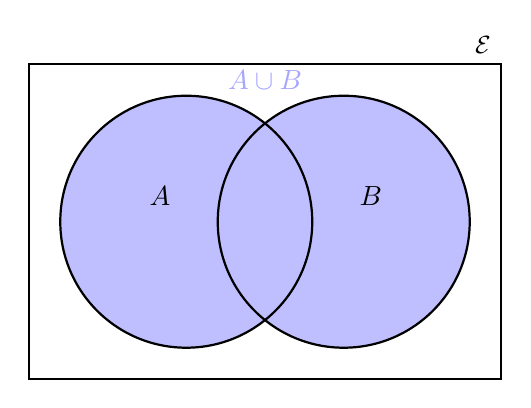
\begin{tikzpicture}[scale=1]
      % Parameters
      \def\R{1.6}
      \coordinate (A) at (-1,0);
      \coordinate (B) at ( 1,0);
    
      % Sample space
      \draw[thick] (-3,-2) rectangle (3,2) node[anchor=south east,font=\small] {$\mathcal{E}$};
    
      % Shade union (fill both circles; overlap appears darker)
      \fill[blue!25] (A) circle (\R);
      \fill[blue!25] (B) circle (\R);
    
      % Outlines and labels
      \draw[thick] (A) circle (\R) node[above left=2pt] {$A$};
      \draw[thick] (B) circle (\R) node[above right=2pt] {$B$};
    
      % Title
      \node[text=blue!35] at (0,1.8) {$A\cup B$};
    \end{tikzpicture}
    \caption{Union $A\cup B$}
    \label{fig:venn-union}
    \end{subfigure}
    \hfill
    \begin{subfigure}[t]{0.47\textwidth}
    \centering
    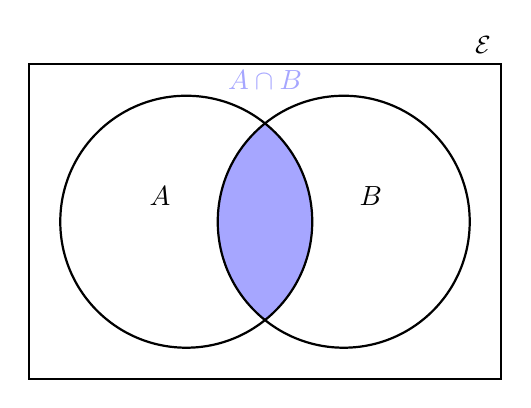
\begin{tikzpicture}[scale=1]
      % Parameters
      \def\R{1.6}
      \coordinate (A) at (-1,0);
      \coordinate (B) at ( 1,0);
    
      % Sample space
      \draw[thick] (-3,-2) rectangle (3,2) node[anchor=south east,font=\small] {$\mathcal{E}$};
    
      % Shade intersection via clipping
      \begin{scope}
        \clip (A) circle (\R);
        \fill[blue!35] (B) circle (\R);
      \end{scope}
    
      % Outlines and labels
      \draw[thick] (A) circle (\R) node[above left=2pt] {$A$};
      \draw[thick] (B) circle (\R) node[above right=2pt] {$B$};
    
      % Title
      \node[text=blue!35] at (0,1.8) {$A\cap B$};
    \end{tikzpicture}
    \caption{Intersection $A\cap B$}
    \label{fig:venn-intersection}
    \end{subfigure}
    
    \caption{Venn diagrams for events \(A\) and \(B\) in sample space $\mathcal{E}$: union and intersection.}
    \label{fig:venn-probability}
\end{figure}

The probability of an event $A$, denoted $P(A)$, is a number in $[0,1]$ that quantifies its likelihood. A useful way to estimate $P(A)$ is via long-run frequency: if we repeat an experiment $N$ times under identical conditions and $A$ occurs $N_A$ times, then $N_A/N$ is an estimate of $P(A)$. In idealized settings, according to the strong law of large numbers, this converges to the true probability as $N \to \infty$:
\begin{equation}
    P(A) = \lim_{N\to\infty} \frac{N_A}{N}
    \label{eq:prob-limit}
\end{equation}
We'll use this frequentist picture for intuition and for simulation results.\footnote{Other interpretations of what ``probability'' means exist. For example, the Bayesian view treats probability as a degree of belief that is updated by data via Bayes' rule. Still, both views use the same axioms and lead to the same calculations for this course.} To avoid circularity, we do not \emph{define} probability by the limit in \autoref{eq:prob-limit}\footnote{This is a bit of a nuance that is not of real consequence to us in 10.34.}. Instead, we take $P(\cdot)$ as a primitive that must obey a few simple rules. These are Kolmogorov's axioms and are listed below.
\begin{definitionBox}
    \textbf{The Axioms of Probability}
    For any events $A_i$ within a sample space $\mathcal{E}$:
    \begin{enumerate}
        \item \textbf{Non-negativity:} The probability of any event is non-negative.
        \begin{equation}
            P(A) \ge 0
        \end{equation}
        \item \textbf{Unity:} The probability of the entire sample space is 1. Some outcome must occur.
        \begin{equation}
            P(\mathcal{E}) = 1
        \end{equation}
        \item \textbf{Additivity:} If events $\{A_i\}_{i=1}^\infty$ are pairwise disjoint,
        \begin{equation}
          P\!\left(\bigcup_{i=1}^\infty A_i\right)=\sum_{i=1}^\infty P(A_i)
        \end{equation}
        For example, if two events are mutually exclusive (i.e., they cannot both occur, $A \cap B = \emptyset$), the probability that either one occurs is  the sum of their individual probabilities: $P(A \cup B) = P(A) + P(B)$. To help visualize this, one can think of this two-event, mutually exclusive case as a figure similar to \autoref{fig:venn-union} but with the two circles non-overlapping. To get the total area of the two circles, the areas can just be added. The non-mutually exlusive case is covered by the law of total probability later on.
    \end{enumerate}
\end{definitionBox}
Note that from these axioms, we immediately have that (1) the probability of the complement of an event $A^{c}$ (the event that $A$ does not occur) is $P(A^{c}) = 1 - P(A)$, and (2) $P(\emptyset) = 0$.
    

\section{Conditional Probability and Independence}
The axioms of probability describe static situations. However, we often need to update our assessment of an event's likelihood in light of new information. The framework for this is \textbf{conditional probability}.

The conditional probability of event $A$ occurring given that event $B$ has occurred is denoted $P(A \mid B)$. Intuitively, knowing that $B$ has happened restricts our sample space from $\mathcal{E}$ to just the outcomes in $B$. The probability of $A$ is then the fraction of this new, smaller sample space that is also occupied by $A$ (\autoref{fig:cond-prob}). This intuition is formalized by the definition:
\begin{equation}
    P(A \mid B) = \frac{P(A \cap B)}{P(B)}, \quad \text{provided } P(B) > 0
    \label{eq:cond-prob}
\end{equation}

\begin{figure}[h]
    \centering
    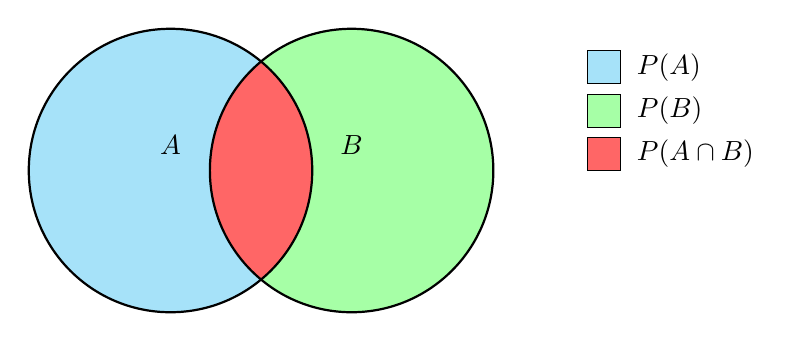
\begin{tikzpicture}
        \def\R{1.8} % circle radius
        \coordinate (A) at (-1.15,0);
        \coordinate (B) at ( 1.15,0);
    
        % --- fills ---
        % base sets
        \fill[cyan!35]  (A) circle (\R);   % A
        \fill[green!35] (B) circle (\R);   % B
        % intersection overlay so it stands out
        \begin{scope}
        \clip (A) circle (\R);
        \fill[red!60] (B) circle (\R);  % A ∩ B
        \end{scope}
    
        % --- outlines and labels for the sets ---
        \draw[thick] (A) circle (\R) node[above=2pt] {$A$};
        \draw[thick] (B) circle (\R) node[above=2pt] {$B$};
    
        % --- legend boxes ---
        \foreach \col/\txt/\y in {
            cyan!35/$P(A)$/1.10,
            green!35/$P(B)$/0.55,
            red!60/$P(A\cap B)$/0.00
        }{
        \fill[\col,draw=black] (4.15,\y) rectangle +(0.42,0.42);
        \node[anchor=west] at (4.65,\y+0.21) {\txt};
        }
        % % --- formula and caption ---
        % \node[anchor=west,align=left] at (7.15,.5) {$P(A\mid B)=\dfrac{P(A\cap B)}{P(B)}$\\[2pt]
        % (restrict sample space to $B$ since it's given)};
    
    \end{tikzpicture}
    \caption{When we condition on $B$, the sample space is restricted to just the $B$ circle, so the probability of $A$ given $B$ is $P(A\mid B)=P(A\cap B)/P(B)$}
    \label{fig:cond-prob}
\end{figure}

The formula in \autoref{eq:cond-prob} is one of the most important in all of probability. By rearranging it, we get the multiplication rule:
\begin{equation}
    P(A \cap B) = P(A \mid B)P(B)
    \label{eq:mult-rule}
\end{equation}

\begin{exampleBox}
    \textbf{Example (Rolling a Die)}: Let's roll a standard six-sided die, so $\mathcal{E} = \{1, 2, 3, 4, 5, 6\}$. Let $A$ be the event of rolling a 3, so $A=\{3\}$, and $B$ be the event of rolling an odd number, so $B=\{1, 3, 5\}$. The unconditional probability is clearly $P(A) = 1/6$. Now, suppose we are told the roll was odd (event $B$). What is the new probability of $A$? The intersection is $A \cap B = \{3\}$, with $P(A \cap B)=1/6$. The probability of our condition is $P(B)=3/6 = 1/2$. Using \autoref{eq:cond-prob}, 
    \begin{equation}
        P(A \mid B) = \frac{P(A \cap B)}{P(B)} = \frac{1/6}{3/6} = \frac{1}{3}
    \end{equation}
    This matches our intuition: once we know the number is odd, there are only three possibilities (1, 3, or 5), each equally likely, so the chance of it being a 3 is $1/3$. Our belief was updated by the new information.
\end{exampleBox}

When the occurrence of one event gives us no information about another, we say the events are \textbf{independent}. We define independence via the product rule:
\begin{equation}
    \text{$A$ and $B$ are independent} \iff P(A \cap B) = P(A)\,P(B)
    \label{eq:prob-independence}
\end{equation}
When $P(B)>0$, this is equivalent to the conditional statement $P(A\mid B)=P(A)$ (and conversely, $P(A\mid B)=P(A)$ together with $P(B)>0$ implies \autoref{eq:prob-independence}). This property extends to any number of \emph{mutually independent} events. Specifically, events $A_1,\dots,A_N$ are mutually independent if for every nonempty subset $\mathcal{I}\subseteq\{1,\dots,N\}$,
\begin{equation}
    P\!\Big(\bigcap_{i\in \mathcal{I}} A_i\Big) = \prod_{i\in \mathcal{I}} P(A_i)
\end{equation}
For example, $P(A\cap B\cap C)=P(A)P(B)P(C)$ holds when $A,B,C$ are mutually independent.

\begin{warningBox}
    \textbf{Warning:} Pairwise independence (every pair independent) does not, in general, imply mutual independence! Here's an example: Toss two fair coins. Let $A=\{\text{first is H}\}$, $B=\{\text{second is H}\}$, and $C=\{\text{coins show the same face}\}$. Then $P(A)=P(B)=P(C)=1/2$ and each pair is independent (e.g., $P(A\cap B)=1/4=P(A)P(B)$, $P(A\cap C)=1/4=P(A)P(C)$, $P(B\cap C)=1/4=P(B)P(C)$), but $P(A\cap B\cap C)=1/4 \neq P(A)P(B)P(C)=1/8$, so $A,B,C$ are pairwise independent yet not mutually independent.
\end{warningBox}

\begin{exampleBox}
    \textbf{Example (Independent Safety Valves)}: A process has three independent safety valves. Each valve has a 5\% chance of being defective. What is the probability that at least one valve is defective?

    Let $D_i$ be the event that valve $i$ is defective. We are given $P(D_i) = 0.05$. The event that a valve works correctly, $W_i$, is the complement, so $P(W_i) = 1 - P(D_i) = 0.95$.

    Calculating the probability of ``at least one defective'' directly is complicated (one fails, or two fail, or all three fail). It is far easier to calculate the probability of the complement event: ``all three valves work correctly.'' Since the valves are independent, we can use \autoref{eq:prob-independence}:
    \begin{equation}
        P(W_1 \cap W_2 \cap W_3) = P(W_1)P(W_2)P(W_3) = (0.95)^3 \approx 0.8574
    \end{equation}
    The event ``at least one valve is defective'' is the complement of ``all three valves work correctly.'' Therefore, its probability is
    \begin{equation}
        P(\text{at least one defective}) = 1 - P(\text{all work}) = 1 - 0.8574 = 0.1426
    \end{equation}
    So, there is a 14.26\% chance that the system has at least one point of failure.
\end{exampleBox}

\subsection{Law of Total Probability}
It is often the case that we might not know $P(B)$ directly, but we can compute the conditional probabilities $P(B \mid A_j)$ and $P(A_j)$ for each $j$. In this case, we can use the law of total probability to compute $P(B)$. Let $\{A_j\}_{j=1}^m$ be a pairwise disjoint ($A_j \cap A_k = \emptyset$ for $j\neq k$) and collectively exhaustive ($\bigcup_{j=1}^m A_j = \mathcal{E}$) partition of the sample space $\mathcal{E}$ with $P(A_j)>0$. For any event $B$,
\begin{equation}
    P(B) = \sum_{j=1}^m P\!\left(B \mid A_j\right)\,P(A_j)
    \label{eq:ltp-events}
\end{equation}

% MC: commenting this out since RVs haven't been discussed yet, and probably jut the above is clear enough
% Equivalently, let $\mathsf{s}$ be a discrete random variable with support $\mathcal{S}=\{s_1,\dots,s_m\}$ (or countable). Then
% \begin{equation}
%   P(B) = \sum_{s\in\mathcal{S}} P\!\left(B \mid \mathsf{s}=s\right)\,P(\mathsf{s}=s)
% \end{equation}
% If $\mathsf{s}$ is continuous with density $p_{\mathsf{s}}(s)$ supported on $\mathcal{S}\subseteq\mathbb{R}^d$, the sum becomes an integral over the support:
% \begin{equation}
%   P(B) = \int_{\mathcal{S}} P\!\left(B \mid \mathsf{s}=s\right)\, p_{\mathsf{s}}(s)\,ds.
%   \label{eq:ltp-cont}
% \end{equation}
% We are basically averaging the conditional probability over the distribution of $\mathsf{s}$.


\subsection{\texorpdfstring{Inclusion-Exclusion and Union Bounds\textsuperscript{*}}{Inclusion-Exclusion and Union Bounds}}
Often, we want the probability that at least one of several events occurs. The Venn diagrams in \Cref{fig:venn-union,fig:venn-intersection} already hint at the key idea: if we simply add $P(A)$ and $P(B)$, we overcount the overlap $A\cap B$, so we must subtract it once. This leads to the \textbf{inclusion-exclusion principle}. The case of two and three events (\autoref{eq:IE-two} and \autoref{eq:IE-three}) are the most common and are likely familiar to you from previous math classes. The general formula is given by \autoref{eq:IE-general}. All the general formula is doing is applying the addition rule repeatedly and then accounting for the overcounting appropriately. In particular, the alternating signs in \autoref{eq:IE-general} correct for overcounting: singles are counted once, pairwise overlaps were counted twice so we subtract them, triple overlaps were then subtracted too many times so we add them back, and so on.

\begin{definitionBox}
\textbf{Inclusion-Exclusion (IE)}. For events $A_1,\dots,A_N$,
\begin{align}
    P(A\cup B) &= P(A)+P(B)-P(A\cap B) \label{eq:IE-two}\\[4pt]
    P(A\cup B\cup C) &= P(A)+P(B)+P(C) \nonumber\\
    &\quad - \big[P(A\cap B)+P(A\cap C)+P(B\cap C)\big] \nonumber\\
    &\quad + P(A\cap B\cap C) \label{eq:IE-three}\\[4pt]
    P\!\Big(\bigcup_{i=1}^N A_i\Big) &= \sum_{i} P(A_i)
    \;-\!\!\sum_{i<j} P(A_i\cap A_j)
    \;+\!\!\sum_{i<j<k} P(A_i\cap A_j\cap A_k)
    \;\mp \cdots \nonumber\\
    &\qquad + (-1)^{r+1}\!\!\!\sum_{i_1<\cdots<i_r}\!\!\! P(A_{i_1}\cap\cdots\cap A_{i_r})
    \;\mp \cdots \nonumber\\
    &\qquad + (-1)^{N+1} P(A_1\cap\cdots\cap A_N)\label{eq:IE-general}
\end{align}
\end{definitionBox}
We note that IE holds without any independence assumptions. Independence is only used, when available, to evaluate the intersections, e.g., $P(A\cap B)=P(A)P(B)$ if $A$ and $B$ are independent. When the events are pairwise disjoint, all intersections vanish and \autoref{eq:IE-two} collapses to the additivity axiom.

\begin{exampleBox}
\textbf{Example: At Least One Defective, Revisited.}
Let $D_1,D_2,D_3$ be the events that each of three safety valves is defective. With independence and $P(D_i)=0.05$,
\begin{gather}
    \sum_i P(D_i)=3(0.05)=0.15 \\
    \sum_{i<j} P(D_i\cap D_j)=3(0.05)^2=0.0075 \\
    P(D_1\cap D_2\cap D_3)=(0.05)^3=0.000125
\end{gather}
By \autoref{eq:IE-three},
\begin{equation}
    P(D_1\cup D_2\cup D_3)=0.15-0.0075+0.000125=0.142625
\end{equation}
which matches the complement calculation $1-(0.95)^3 \approx 0.142625$ from earlier.
\end{exampleBox}

\paragraph*{\texorpdfstring{Union bounds and Bonferroni inequalities\textsuperscript{*}}{Union bounds and Bonferroni inequalities}}
Exact IE can be tedious for large $N$. Truncating \autoref{eq:IE-general} gives us useful bounds, known as Bonferroni inequalities. Keeping only the first (positive) term gives the union bound (a.k.a.\ Boole's inequality):
\begin{equation}
    P\!\Big(\bigcup_{i=1}^N A_i\Big) \le \sum_{i=1}^N P(A_i)
    \label{eq:union-bound}
\end{equation}
Including the pairwise term gives a lower bound:
\begin{equation}
    P\!\Big(\bigcup_{i=1}^N A_i\Big) \ge \sum_i P(A_i) - \sum_{i<j} P(A_i\cap A_j)
    \label{eq:bonferroni-lb}
\end{equation}
More generally, truncating after an odd number of terms gives an upper bound, while truncating after an even number gives a lower bound. We emphasize that these bounds follow directly from \autoref{eq:IE-general}.

\begin{exampleBox}
\textbf{Example: Quick Estimate with a Union Bound.}
If sensors $S_1,\dots,S_5$ have false-alarm probabilities at most $1\%$ each, then
\begin{equation}
    P(\text{at least one false alarm}) \le \sum_{i=1}^5 0.01 = 0.05
\end{equation}
This bound is immediate and does not require independence.
\end{exampleBox}
The takeaway here is to use \autoref{eq:IE-two}-\autoref{eq:IE-general} for exact computations when intersections are accessible (by symmetry, structure, or independence). When they are not, \autoref{eq:union-bound} and \autoref{eq:bonferroni-lb} provide fast, informative bounds. The pictures in \Cref{fig:venn-union,fig:venn-intersection} are a helpful guide to remember the alternating-sign corrections.


\subsection{Simpson's paradox}
Conditional probability can lead to counterintuitive results when we fail to account for all relevant information. \textbf{Simpson's paradox} occurs when a trend appears in different groups of data but disappears or reverses when the groups are combined. When a confounding variable influences both the condition and the outcome, ignoring this variable can lead to misleading conclusions. It's easiest to see this with an example.

\begin{exampleBox}
    \textbf{Example (Simpson's Paradox):}
    Let $x$ denote weekly exercise hours, $y$ resting blood pressure, and $S\in\{\text{Younger (A)},\text{Older (B)}\}$ indicate age group. In the scatter of \autoref{fig:simpsons-scatter}, each age group shows the expected \emph{negative} association: within a fixed age group, more exercise is linked to lower blood pressure. However, when the groups are pooled and the age indicator $S$ is omitted,
    \begin{equation}
        y = \alpha + \beta x + \varepsilon,\quad \beta>0
    \end{equation}
    so exercise appears (misleadingly) to increase blood pressure. The reversal occurs because age is a confounder: older adults (group B) both exercise more on average ($x$ larger) and have higher baseline blood pressure ($\alpha_B>\alpha_A$). This shift in intercepts and in the distribution of $x$ across groups means that
    \begin{equation}
        \operatorname{sign}\!\left(\operatorname{Cov}(x,y\mid S=s)\right)<0
        \quad\text{but}\quad
        \operatorname{sign}\!\left(\operatorname{Cov}(x,y)\right)>0
    \end{equation}
    We can see then how important it is to condition on the relevant variables.

    \begin{figure}[H]
      \centering
      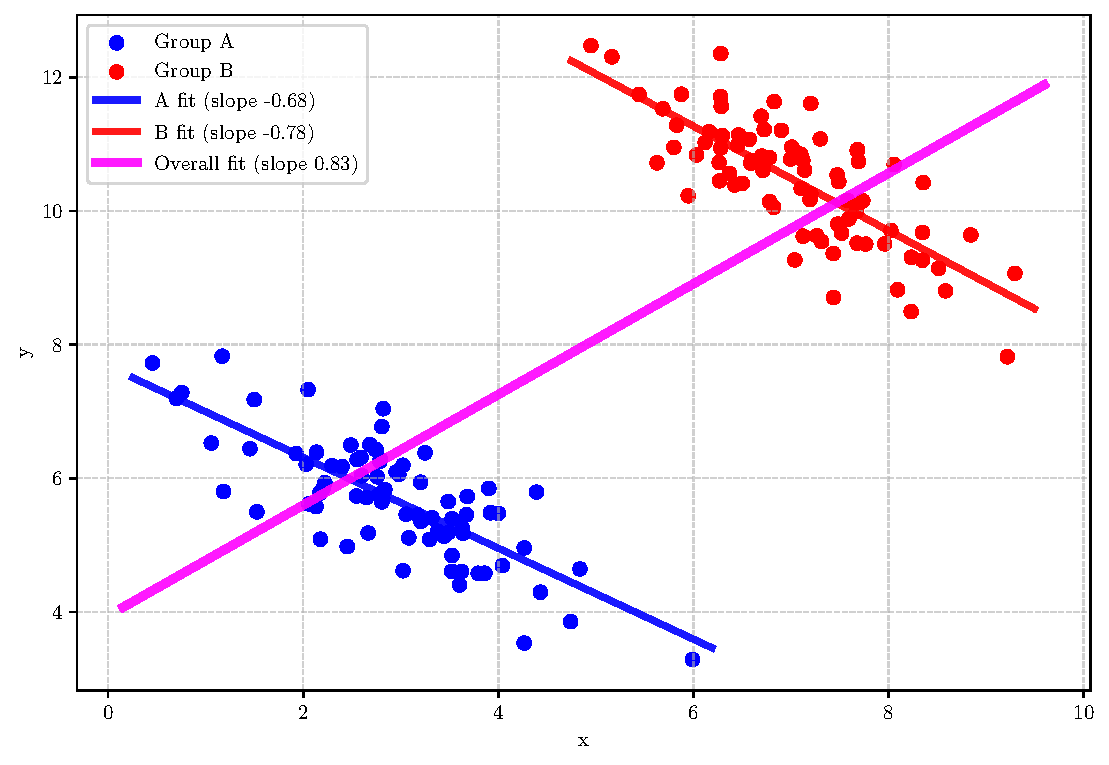
\includegraphics[width=\linewidth]{figs/probability/simpsons_paradox_scatter.pdf}
      \caption{Simpson's paradox in a continuous setting. Within each age group (A: younger, B: older) the fitted slope is negative; pooled across groups the fitted slope is positive.}
      \label{fig:simpsons-scatter}
    \end{figure}
    
\end{exampleBox}
    
The main message to get across here is that when analyzing data, we must carefully consider what variables to condition on. If important conditioning variables are omitted from the analysis, the results can be completely misleading. Always consider what additional information might be relevant to properly interpret probabilistic relationships.

\subsection{Bayes' Theorem}
The law of total probability allows us to synthesize the probability of an effect ($D$) from various potential causes ($A, B, C$). But what if we observe the effect and want to infer the cause? For instance, if we find a defective part, what is the probability that it came from Machine A? We are looking to invert the conditional probability from $P(\text{Effect} \mid \text{Cause})$ to $P(\text{Cause} \mid \text{Effect})$. This is the purpose of \textbf{Bayes' theorem}.

The theorem is a direct consequence of the definition of conditional probability. From the multiplication rule, we have two ways of expressing the intersection $A_i \cap B$:
\begin{align*}
    P(A_i \cap B) &= P(B \mid A_i)P(A_i) \\
    P(A_i \cap B) &= P(A_i\mid B)P(B)
\end{align*}
Setting these equal and rearranging to solve for $P(A_i \mid B)$ gives the simple form of Bayes' theorem (assuming $P(B)>0$):
\begin{equation}
    P(A_i \mid B) = \frac{P(B \mid A_i)P(A_i)}{P(B)}
    \label{eq:bayes-simple}
\end{equation}
A lot of the time, we don't know $P(B)$ directly, so we expand it via the law of total probability. This gives us the full form of Bayes' theorem:
\begin{definitionBox}
    \textbf{Bayes' Theorem.} Let $\{A_j\}$ be a partition of the sample space (mutually exclusive and collectively exhaustive) with $P(A_j)>0$, and let $P(B)>0$. Then
    \begin{equation}
        P(A_i \mid B) = \frac{P(B \mid A_i)P(A_i)}{\sum_{j} P(B \mid A_j)P(A_j)}
        \label{eq:bayes-full}
    \end{equation}
\end{definitionBox}
This formula provides a systematic way to update our beliefs in light of new evidence. The terms have special names that reflect this process:
\begin{itemize}
    \item $P(A_i)$ is the \textbf{prior probability}: our initial belief about the cause before seeing any evidence.
    \item $P(B \mid A_i)$ is the \textbf{likelihood}: the probability of observing the evidence $B$ if the cause $A_i$ were true.
    \item $P(A_i \mid B)$ is the \textbf{posterior probability}: our updated belief about the cause after observing the evidence.
    \item $P(B)$ is the \textbf{marginal likelihood} of the evidence (also just called the evidence), which serves as a normalization constant.
\end{itemize}

\begin{exampleBox}
    \textbf{Example (Manufacturing Defects, continued)}: We found that the overall defect rate was $P(D) = 0.021$. Now, suppose we have a defective part in hand. What is the probability it came from Machine B, i.e., what is $P(B\mid D)$?

    Our prior belief was $P(B) = 0.35$. We now use Bayes' Theorem to update this belief with the evidence that the part is defective.
    \begin{equation}
        P(B \mid D) = \frac{P(D \mid B)P(B)}{P(D)}
    \end{equation}
    We have all the necessary components: $P(D \mid B)=0.03$, $P(B)=0.35$, and $P(D)=0.021$. So
    \begin{equation}
        P(B \mid D) = \frac{0.03 \times 0.35}{0.021} = \frac{0.0105}{0.021} = 0.5
    \end{equation}
    After finding a defective part, the probability that it came from Machine B has increased from 35\% (the prior) to 50\% (the posterior). This is because Machine B has the highest defect rate, so it is disproportionately responsible for the defective parts.
\end{exampleBox}

\begin{exampleBox}
    \textbf{Example (Diagnostic Testing)}: A diagnostic test for pipeline corrosion has a sensitivity of 85\% (it correctly identifies corrosion 85\% of the time) and a specificity of 99.9\% (it correctly reports no corrosion 99.9\% of the time). Industry data suggests that this corrosion is present in 1\% of pipes of a certain age. If a pipe tests positive, what is the probability it actually has corrosion?

    Let $C$ be the event the pipe has corrosion, and $C^c$ be the event it does not. Let $T^+$ be a positive test result. We are given the prior that $P(C) = 0.01$, so $P(C^c) = 0.99$. We also know that the sensitivity is $P(T^+ \mid C)=0.85$, and the specificity is $P(T^- \mid C^c)=0.999$, which implies a false positive rate of $P(T^+ \mid C^c) = 1 - 0.999 = 0.001$.

    We want to find the posterior, $P(C \mid T^+)$. Using Bayes' Theorem (\autoref{eq:bayes-full}):
    \begin{equation}
        P(C \mid T^+) = \frac{P(T^+ \mid C)P(C)}{P(T^+ \mid C)P(C) + P(T^+ \mid C^c)P(C^c)}
    \end{equation}
    Plugging in the numbers:
    \begin{equation}
        P(C \mid T^+) = \frac{0.85 \times 0.01}{0.85 \times 0.01 + 0.001 \times 0.99} = \frac{0.0085}{0.0085 + 0.00099} = \frac{0.0085}{0.00949} \approx 0.896
    \end{equation}
    Despite strong test characteristics, a positive result has a posterior below 100\% ($\approx 89.6\%$) because the prior prevalence is only 1\%. The base rate still materially limits certainty.
\end{exampleBox}

\section{Random Variables}
So far, we have worked with events defined on a sample space $\mathcal{E}$. The outcomes in $\mathcal{E}$ can be numerical (like the result of a die roll) or categorical (like ``heads'' or ``defective''). To unify the analysis of these experiments, we introduce the concept of a \textbf{random variable (RV)}, which provides a consistent way to assign a numerical value to every possible outcome. Formally, a random variable is a function that maps an outcome from the sample space $\mathcal{E}$ to a real number.

We make a brief note on notation: To distinguish between the RV itself (which is a function) and the specific values it can take, we will adopt the convention that an RV will be denoted with a sans-serif font, like $\mathsf{x}$ or $\mathsf{t}$, while a specific, single value that the random variable takes after a trial (known as a \emph{realization}) will be denoted with a standard italic font, like $x$ or $t$. So, if $\xi$ is the outcome of a particular trial, $x = \mathsf{x}(\xi)$ is the numerical value assigned to that outcome by the RV $\mathsf{x}$.

The primary utility of a random variable is that it allows us to define events using numerical statements. For example, instead of describing a complex set of outcomes, we can make a simple statement like ``the temperature is greater than 400 K.'' This translates an event in the numerical space back to a corresponding event in the original sample space:
\begin{equation}
    P(\mathsf{x} \ge a) := P(\{\xi \in \mathcal{E} \mid \mathsf{x}(\xi) \ge a\})
\end{equation}

Random variables are usually classified into two types based on the values they can take. \textbf{Discrete random variables} can take on a finite or countably infinite number of distinct values. For example, we can use a discrete RV to describe the result of a coin flip: $\mathsf{x}$ such that $\mathsf{x}(\text{heads}) = 1$ and $\mathsf{x}(\text{tails}) = 0$. Here, the set of possible values is $\{0, 1\}$. Meanwhile, \textbf{continuous random variables} can take on any value within a given continuous range. The number of possible values is uncountably infinite. For example, consider the measured temperature of a reactor, $\mathsf{T}$, which can be any value in $[0, \infty)$. In such cases, single points have probability zero: $P(\mathsf{T}=t)=0$. Understanding the type of a random variable is the first step toward describing its behavior using a probability distribution, which we will cover next.

\section{CDFs, PMFs, and PDFs}
Random variables give us a tool to map experimental outcomes to numbers. The next step is to describe the probabilistic behavior of that variable. We need to answer the question: ``What are the probabilities that the random variable $\mathsf{x}$ will take on certain values?'' This is the role of a \textbf{probability distribution}. There are two main functions we use to fully characterize a random variable's distribution. One is universal, while the other is specific to whether the variable is discrete or continuous.

\paragraph*{Support}
We write $\mathcal{S}_{\mathsf{x}}$ for the support of $\mathsf{x}$, i.e., the set of values where the distribution puts positive probability (discrete) or positive density (continuous).

% TODO: add TikZ sketches for CDF, PMF, and PDF
\subsection{The Cumulative Distribution Function}
The most fundamental description of any random variable's distribution is the \textbf{cumulative distribution function (CDF)}. The CDF, denoted by $F_{\mathsf{x}}(x)$, is defined as the probability that the random variable $\mathsf{x}$ takes on a value less than or equal to a specific value $x$.
\begin{equation}
    F_{\mathsf{x}}(x) = P(\mathsf{x} \le x)
    \label{eq:cdf-def}
\end{equation}
The CDF accumulates probability as $x$ increases. By definition, it is a non-decreasing function that starts at 0 for $x \to -\infty$ and ends at 1 for $x \to +\infty$; it should be obvious why these limits are necessary given the axioms of probability. A consequence of \autoref{eq:cdf-def} is that for any $a<b$,
\begin{equation}
    P(a<\mathsf{x}\le b)=F_{\mathsf{x}}(b)-F_{\mathsf{x}}(a)
    \label{eq:cdf-range}
\end{equation}
The use of $<$ and $\le$ is very deliberate here: the CDF is right-continuous, but not necessarily left-continuous. Only if the CDF is (fully) continuous at $a$ and $b$ are we allowed to switch both bounds to $\le$.

\subsection{The Probability Mass Function for Discrete RVs}
For a discrete random variable, it's most intuitive to describe the ``lump'' of probability at each specific value it can take. This is the job of the \textbf{probability mass function (PMF)}, denoted by $p_{\mathsf{x}}(x)$.
\begin{equation}
    p_{\mathsf{x}}(x) = P(\mathsf{x} = x)
    \label{eq:pmf-def}
\end{equation}
The PMF gives a probability for each possible outcome. It must satisfy two conditions: $p_{\mathsf{x}}(x) \ge 0$ for all $x$, and the sum over all possible values in its support must be 1: $\sum_{x \in \mathcal{S}_{\mathsf{x}}} p_{\mathsf{x}}(x) = 1$. The PMF links to the CDF via
\begin{equation}
    F_{\mathsf{x}}(x) = \sum_{a \le x} p_{\mathsf{x}}(a)
\end{equation}

\subsection{The Probability Density Function for Continuous RVs}
For a continuous random variable, the situation is more subtle. Since there are infinitely many possible values in any range, the probability of the RV taking on any single, exact value is zero. For example, $P(\mathsf{T} = 373.150000... \text{ K}) = 0$. Instead, we talk about the probability of the variable falling within a range $[a,b]$. We describe this using a \textbf{probability density function (PDF)}. We'll again use $p_{\mathsf{x}}(x)$ to denote a PDF; context will make clear whether it's a PMF or PDF. The PDF is the function we integrate to find the probability of being in a range:
\begin{equation}
    P(a \le \mathsf{x} \le b) = \int_{a}^{b} p_{\mathsf{x}}(x)\,dx
    \label{eq:pdf-range}
\end{equation}
Like the PMF, the PDF must be non-negative, $p_{\mathsf{x}}(x) \ge 0$, and its total integral must be 1: $\int_{-\infty}^{\infty} p_{\mathsf{x}}(x)\,dx = 1$. We take the support to be $\mathcal{S}_{\mathsf{x}}=\{x: p_{\mathsf{x}}(x)>0\}$, and probabilities of intervals outside $\mathcal{S}_{\mathsf{x}}$ are zero. Assuming the PDF exists and is continuous (which is not always true), the PDF links to the CDF via
\begin{equation}
    F_{\mathsf{x}}(x) = \int_{-\infty}^{x} p_{\mathsf{x}}(t)\,dt \iff p_{\mathsf{x}}(x) = \frac{d}{dx}F_{\mathsf{x}}(x)
\end{equation}

\begin{warningBox}
    \textbf{Warning: PDF Danger Zone.}\quad Here are two points to watch out for when working with PDFs:
    \begin{enumerate}
        \item A PDF value is not a probability. Unlike a PMF, the value of a PDF, $p_{\mathsf{x}}(x)$, is a probability density. It can be greater than 1. The probability is the area under the curve. For a very small interval, the probability is approximately the area of a rectangle: $P(x \le \mathsf{x} \le x+dx) \approx p_{\mathsf{x}}(x)dx$.
        \item The probability at a point is zero (if in doubt, check out \autoref{eq:pdf-range} and realize that you would be integrating over a zero-width interval). For any continuous RV, $P(\mathsf{x}=c)=0$. This means that $P(a \le \mathsf{x} \le b)$ is the same as $P(a < \mathsf{x} < b)$.
    \end{enumerate}
\end{warningBox}

\section{Sampling and Expectations}
% MC: seems like sampling doesn't come up in this section so maybe should retitle and remove intro about sampling
% or rewrite to discuss sampling first
The link between a theoretical probability distribution and real-world data is \textbf{sampling}. When we perform an experiment and get a realization $x$ of a random variable $\mathsf{x}$, we are ``drawing a sample'' from its distribution. With independent and identically distributed sampling, relative frequencies (discrete) converge to the true probabilities, and histograms/density estimators (continuous) approximate the PDF as the sample size grows. This connects our formal definitions back to the intuitive idea of probability as long-run frequency. When we get these distributions (empirically or theoretically), we get a complete, but sometimes overwhelmingly detailed, description of a random variable. We often want to summarize a distribution with a few key numbers that describe its central tendency, spread, and shape. We will cover some of these below and see how they can be estimated from sample data.

\paragraph*{The Expected Value (Mean)}
The most important summary statistic is the \textbf{expected value} (also known as the expectation or the mean). It represents the long-run average value of the random variable over many trials. It is the center of mass of the distribution. The expectation operator is denoted by $\mathbb{E}[\cdot]$ or angle brackets $\langle\cdot\rangle$. For a discrete RV,
\begin{equation}
    \mu_{\mathsf{x}} = \mathbb{E}[\mathsf{x}] = \sum_{x} x \, p_{\mathsf{x}}(x) \qquad\text{(discrete)}
\end{equation}
And for a continuous RV,
\begin{equation}
    \mu_{\mathsf{x}} = \mathbb{E}[\mathsf{x}] = \int_{-\infty}^{\infty} x \, p_{\mathsf{x}}(x)\,dx \qquad\text{(continuous)}
\end{equation}
These integrals/sums assume the expectation exists (is finite).

% MC: we can delete these boxes to avoid confusion
The below warning and example are both a little beyond the scope of 10.34, but it's something you should be aware of since you'll see it in the literature all the time.
\begin{warningBox}
    \textbf{Warning:} If you're keeping track of multiple variables, it helps to explicitly specify what the expectation is over. Use $\mathbb{E}_\mathsf{x}[\cdot]$ to indicate expectation with respect to $p_\mathsf{x}$, and $\mathbb{E}[\cdot \mid \mathsf{y}]$ for the conditional under $p_{\mathsf{x}\mid \mathsf{y}}$. If other variables are random, either condition on them or integrate them out; don't silently treat them as fixed. Recall that $\mathsf{x}$ (a random variable) is distinct from a realized value $x$.
\end{warningBox}

\begin{exampleBox}
    \textbf{Example:} Let's take a look at an example of explicitly specifying what the expectation is over from the paper \href{https://arxiv.org/abs/2006.11239}{Denoising Diffusion Probabilistic Models} by Ho et al. We keep the notation of the paper here (notice how they don't use sans serif for the random variables, etc.---this is very common in the literature and is generally accepted by the community). In the paper, the simplified training loss is
    \begin{equation}
    L_{\text{simple}}(\theta)
    =\mathbb{E}_{t,x_0,\varepsilon}\!\left[
    \left\|\varepsilon-\varepsilon_\theta\!\left(\sqrt{\bar\alpha_t}\,x_0+\sqrt{1-\bar\alpha_t}\,\varepsilon,\,t\right)\right\|^2
    \right]
    \end{equation}
    Here, $t\sim\mathrm{Unif}\{1,\dots,T\}$ (discrete uniform distribution), $x_0\sim q(x_0)$ is a random data point, and $\varepsilon\sim\mathcal{N}(0,I)$. Thus, $\mathbb{E}_{t,x_0,\varepsilon}[\cdot]$ averages jointly over these three sources of randomness. If we instead \emph{condition} on a fixed datapoint, we write
    \begin{equation}
    \mathbb{E}\!\left[\cdot \mid x_0\right]=\mathbb{E}_{t,\varepsilon}\!\left[\cdot \,\big|\, x_0\right]
    \end{equation}
    so the expectation is only over $t$ and $\varepsilon$ while $x_0$ is held fixed. Likewise, a single reverse-process term can be written as
    \begin{equation}
    L_{t-1}
    =\mathbb{E}_{x_0,\varepsilon}\!\left[
    \frac{\beta_t^2}{2\sigma_t^2\alpha_t(1-\bar\alpha_t)}
    \left\|\varepsilon-\varepsilon_\theta\!\left(\sqrt{\bar\alpha_t}\,x_0+\sqrt{1-\bar\alpha_t}\,\varepsilon,\,t\right)\right\|^2
    \right]+C
    \end{equation}
    making explicit that the averaging is with respect to the data $x_0$ and the Gaussian noise $\varepsilon$, with constants collected in $C$.
\end{exampleBox}
    
    
\paragraph*{Expectation of a Function of an RV}
We can also calculate the expected value of a function of a random variable, $g(\mathsf{x})$. For a discrete RV,
\begin{equation}
\mathbb{E}[g(\mathsf{x})] = \sum_{x} g(x) \, p_{\mathsf{x}}(x) \qquad\text{(discrete)}
\end{equation}
And for a continuous RV,
\begin{equation}
\mathbb{E}[g(\mathsf{x})] = \int_{-\infty}^{\infty} g(x) \, p_{\mathsf{x}}(x)\,dx \qquad\text{(continuous)}
\end{equation}
These formulas are often referred to as the law of the unconscious statistician (commonly known as LOTUS). A very important property is that expectation is a linear operator, meaning $\mathbb{E}[a\mathsf{x} + b] = a\mathbb{E}[\mathsf{x}] + b$. However, for a general nonlinear function $g$, it is \emph{not} true that $\mathbb{E}[g(\mathsf{x})] = g(\mathbb{E}[\mathsf{x}])$.

\begin{exampleBox}
    \textbf{Example ($\mathbb{E}[g(\mathsf{x})] \neq g(\mathbb{E}[\mathsf{x}])$)}: Consider rolling a fair six-sided die. The RV $\mathsf{x}$ can take values $\{1, 2, 3, 4, 5, 6\}$, each with $p_{\mathsf{x}}(x)=1/6$. The expected value is $\mathbb{E}[\mathsf{x}] = (1+2+3+4+5+6)/6 = 3.5$.
    Now, let's consider the function $g(x) = x^2$. What is $\mathbb{E}[\mathsf{x}^2]$?
    $$ \mathbb{E}[\mathsf{x}^2] = \sum_{x=1}^{6} x^2 p_{\mathsf{x}}(x) = \frac{1}{6}(1^2 + 2^2 + 3^2 + 4^2 + 5^2 + 6^2) = \frac{91}{6} \approx 15.17 $$
    However, $g(\mathbb{E}[\mathsf{x}]) = (\mathbb{E}[\mathsf{x}])^2 = (3.5)^2 = 12.25$. As we can see, $\mathbb{E}[\mathsf{x}^2] \neq (\mathbb{E}[\mathsf{x}])^2$.
\end{exampleBox}

\paragraph*{Variance and Standard Deviation}
The \textbf{variance} measures the spread or dispersion of a distribution around its mean. It is defined as the expected squared deviation from the mean.
\begin{equation}
    \sigma_{\mathsf{x}}^2 = \operatorname{Var}(\mathsf{x}) = \mathbb{E}\big[(\mathsf{x} - \mu_{\mathsf{x}})^2\big]
\end{equation}
A more convenient formula for computation can be derived using the linearity of expectation:
\begin{align}
    \sigma_{\mathsf{x}}^2 &= \mathbb{E}[(\mathsf{x} - \mathbb{E}[\mathsf{x}])^2] \nonumber \\
    &= \mathbb{E}[\mathsf{x}^2 - 2\mathsf{x}\mathbb{E}[\mathsf{x}] + (\mathbb{E}[\mathsf{x}])^2] \nonumber\\
    &= \mathbb{E}[\mathsf{x}^2] - \mathbb{E}[2\mathsf{x}\mathbb{E}[\mathsf{x}]] + \mathbb{E}[(\mathbb{E}[\mathsf{x}])^2] \quad (\text{by linearity}) \nonumber\\
    &= \mathbb{E}[\mathsf{x}^2] - 2\mathbb{E}[\mathsf{x}]\mathbb{E}[\mathsf{x}] + (\mathbb{E}[\mathsf{x}])^2 \quad (\text{since } \mathbb{E}[\mathsf{x}] \text{ is a constant}) \nonumber\\
    &= \mathbb{E}[\mathsf{x}^2] - (\mathbb{E}[\mathsf{x}])^2
\end{align}
The \textbf{standard deviation}, $\sigma_{\mathsf{x}} = \sqrt{\operatorname{Var}(\mathsf{x})}$, is the square root of the variance and has the same units as the random variable itself. Other properties like skewness (asymmetry) and kurtosis (tailedness) are defined by higher-order centered moments.

\paragraph*{\texorpdfstring{Law of Iterated Expectations\textsuperscript{*}}{Law of Iterated Expectations}}
For random variables $\mathsf{x}$ and $\mathsf{s}$,
\begin{equation}
  \mathbb{E}[\mathsf{x}] = \mathbb{E}\left[\mathbb{E}[\mathsf{x}\mid \mathsf{s}]\right]
  \label{eq:lie}
\end{equation}
In words, this means that we first average the conditional mean within each group $\mathsf{s}$, then average across groups with the distribution of $\mathsf{s}$. In discrete form,
\begin{equation}
  \mathbb{E}[\mathsf{x}]=\sum_j \mathbb{E}\left[\mathsf{x}\mid \mathsf{s}=s_j\right]\,P(\mathsf{s}=s_j)
\end{equation}
where the sum runs over the support of $\mathsf{s}$. In continuous form with $\mathcal{S}_\mathsf{s}$ being the support of $\mathsf{s}$,
\begin{equation}
  \mathbb{E}[\mathsf{x}]=\int_{\mathcal{S}_\mathsf{s}} \mathbb{E}\left[\mathsf{x}\mid \mathsf{s}=s\right]\,p_{\mathsf{s}}(s)\,ds
\end{equation}
The intuition behind LIE is that the conditional expectation $\mathbb{E}[\mathsf{x}\mid \mathsf{s}]$ is the best mean-squared-error predictor of $\mathsf{x}$ when $\mathsf{s}$ is known exactly. Before seeing $\mathsf{s}$, the random variable $\mathbb{E}[\mathsf{x}\mid \mathsf{s}]$ reflects our best guess for each possible value of $\mathsf{s}$. Averaging these guesses with the natural probabilities of $\mathsf{s}$ returns the overall best uninformed guess, $\mathbb{E}[\mathsf{x}]$.

\begin{exampleBox}
    \textbf{Example: Hits by Scaffold.}
    In a small-molecule generator, each proposal is first sampled by scaffold cluster $\mathsf{s}\in\{\text{A},\text{B},\text{C}\}$ and then instantiated with substituents. Let $\mathsf{h}\in\{0,1\}$ indicate whether the molecule hits (e.g., passes a docking/physics threshold). By construction, the scaffold determines the conditional hit rate $p_{\text{hit}}(s)=\mathbb{E}[\mathsf{h}\mid \mathsf{s}=s]$. Suppose the generator samples scaffolds with
    \begin{equation}
        P(\mathsf{s}=\text{A})=0.5,\quad P(\mathsf{s}=\text{B})=0.3,\quad P(\mathsf{s}=\text{C})=0.2
    \end{equation}
    and the conditional hit rates (estimated from prior campaigns or a calibrated surrogate) are
    \begin{equation}
        p_{\text{hit}}(\text{A})=0.008,\quad p_{\text{hit}}(\text{B})=0.021,\quad p_{\text{hit}}(\text{C})=0.003
    \end{equation}
    The law of iterated expectations gives the overall hit probability for a random proposal,
    \begin{equation}
        \mathbb{E}[\mathsf{h}]
        = \mathbb{E}\left[\mathbb{E}[\mathsf{h}\mid \mathsf{s}]\right]
        = \sum_{s\in\{\text{A,B,C}\}} p_{\text{hit}}(s)\,P(\mathsf{s}=s)
        = (0.008)(0.5)+(0.021)(0.3)+(0.003)(0.2)=0.0109
    \end{equation}
    Thus the expected hit rate is $1.09\%$. By linearity, for a batch of $N$ proposals, the expected number of hits is
    \begin{equation}
        \mathbb{E}[\text{hits in batch}] = N\,\mathbb{E}[\mathsf{h}] = 0.0109 \,N
    \end{equation}
    e.g., with $N=2000$, $\mathbb{E}[\text{hits}]=21.8\approx 22$.
\end{exampleBox}
  

\paragraph*{\texorpdfstring{Law of Total Variance\textsuperscript{*}}{Law of Total Variance}}
For the same $\mathsf{x}$ and $\mathsf{s}$,
\begin{equation}
  \operatorname{Var}(\mathsf{x})
  =
  \mathbb{E}\left[\operatorname{Var}(\mathsf{x}\mid \mathsf{s})\right]
  +
  \operatorname{Var}\left(\mathbb{E}[\mathsf{x}\mid \mathsf{s}]\right)
  \label{eq:ltv}
\end{equation}
We can interpret each term as follows:
\begin{itemize}
  \item $\mathbb{E}[\operatorname{Var}(\mathsf{x}\mid \mathsf{s})]$: average \emph{within-group} variability (irreducible noise once $\mathsf{s}$ is known).
  \item $\operatorname{Var}(\mathbb{E}[\mathsf{x}\mid \mathsf{s}])$: \emph{between-group} variability (how group means differ across $\mathsf{s}$).
\end{itemize}
% TODO: add good, illustrative examples

\section{Some Notable Probability Distributions}
While there are countless probability distributions, a small number of them appear so frequently in science and engineering that they deserve special attention. They serve as fundamental building blocks for modeling a vast range of stochastic phenomena.

\paragraph*{The Binomial Distribution}
The binomial distribution is a discrete distribution that answers the question: ``If I run $n$ independent trials, each with a success probability of $p$, what is the probability of getting exactly $k$ successes?'' It's used for modeling binary outcomes (yes/no, success/failure, on/off) in a fixed number of trials.

Let $\mathsf{k}$ be the random variable for the number of successes. The PMF is given by
\begin{equation}
    p_{\mathsf{k}}(k) = \binom{n}{k} p^k (1-p)^{n-k} \quad \text{for } k \in \{0, 1, \dots, n\}
\end{equation}
This formula combines the probability of one specific sequence of $k$ successes and $n-k$ failures, $p^k(1-p)^{n-k}$, with the number of ways that sequence can occur, given by the binomial coefficient $\binom{n}{k} = n!/(k!(n-k)!)$.

% MC: was using minipage but using this hack to get vertical centering. looks better imo
\begin{tabular}{@{}>{\raggedright\arraybackslash}m{0.48\textwidth} >{\raggedleft\arraybackslash}m{0.48\textwidth}@{}}
    \begin{itemize}
        \item \textbf{Notation}: $\mathsf{k} \sim B(n, p)$
        \item \textbf{Mean}: $\mathbb{E}[\mathsf{k}] = np$
        \item \textbf{Variance}: $\operatorname{Var}(\mathsf{k}) = np(1-p)$
        \item \textbf{Support}: $\mathsf{k} \in \{0, 1, \dots, n\} = \mathbb{Z}_{\ge 0}$
    \end{itemize}
    &
    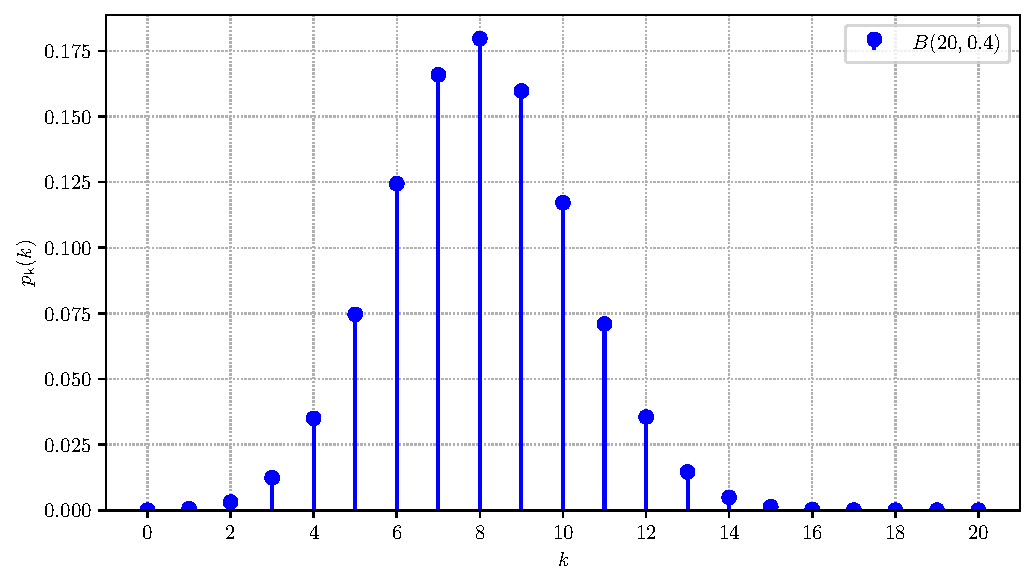
\includegraphics[width=\linewidth]{figs/probability/binomial_pmf.pdf} \\
\end{tabular}


\paragraph*{The Uniform Distribution}
The uniform distribution is the simplest continuous distribution. It describes a situation of complete uncertainty over a fixed interval $[a, b]$, where the probability of the outcome falling in any sub-interval is proportional only to the length of that sub-interval. Every value within the range is equally likely. 

The PDF is a simple constant function:
\begin{equation}
    p_{\mathsf{x}}(x) = 
    \begin{cases} 
        \dfrac{1}{b-a} & \text{for } a \le x \le b \\[2ex]
        0 & \text{otherwise}
    \end{cases}
\end{equation}
The height of the PDF, $1/(b-a)$, is set to ensure that the total area under the curve is equal to 1.

\begin{tabular}{@{}>{\raggedright\arraybackslash}m{0.48\textwidth} >{\raggedleft\arraybackslash}m{0.48\textwidth}@{}}
    \begin{itemize}
        \item \textbf{Notation}: $\mathsf{x} \sim \mathcal{U}(a, b)$
        \item \textbf{Mean}: $\mathbb{E}[\mathsf{x}] = \dfrac{a+b}{2}$
        \item \textbf{Variance}: $\operatorname{Var}(\mathsf{x}) = \dfrac{(b-a)^2}{12}$
        \item \textbf{Support}: $\mathsf{x} \in [a, b]$
    \end{itemize}
    &
    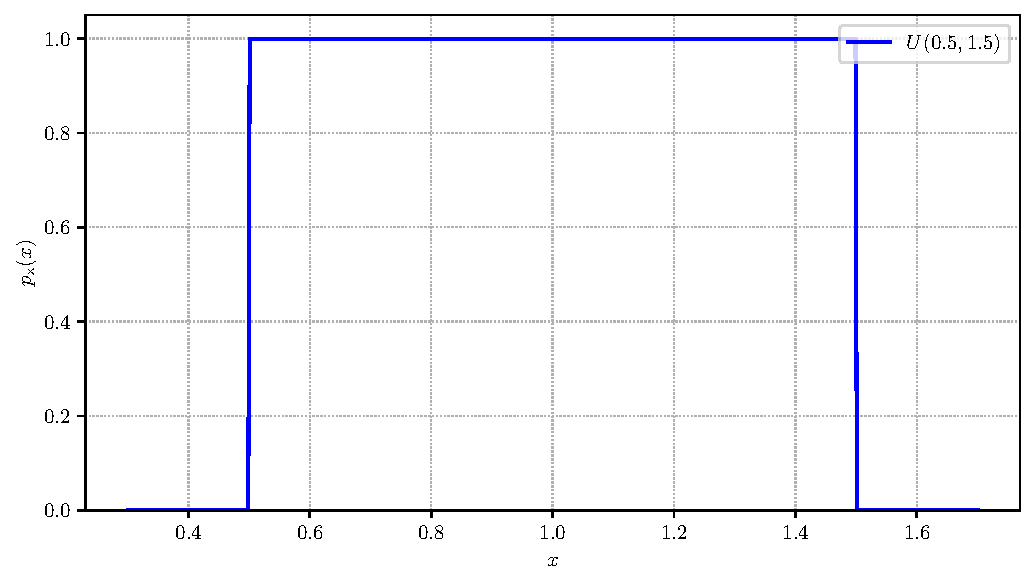
\includegraphics[width=\linewidth]{figs/probability/uniform_pdf.pdf} \\
\end{tabular}

\paragraph*{The Normal (Gaussian) Distribution}
The normal distribution, also known as the Gaussian distribution, is arguably the most important continuous distribution in all of probability and statistics. Its importance comes from the central limit theorem, which states that the sum of a large number of independent random variables will be approximately normally distributed, regardless of their individual distributions (we'll discuss this in more detail later). This is why it appears everywhere. It is the classic ``bell curve.'' 

The PDF is parameterized by the mean $\mu$ and the variance $\sigma^2$:
\begin{equation}
    p_{\mathsf{x}}(x) = \frac{1}{\sigma\sqrt{2\pi}} \exp\left(-\frac{(x-\mu)^2}{2\sigma^2}\right)
\end{equation}
The mean $\mu$ sets the center of the peak, and the standard deviation $\sigma$ controls the spread of the curve. The special case where $\mu=0$ and $\sigma^2=1$ is called the \textbf{standard normal distribution}. Any normal random variable can be converted to a standard normal by the transformation $\mathsf{z} = (\mathsf{x}-\mu)/\sigma$.

\begin{tabular}{@{}>{\raggedright\arraybackslash}m{0.48\textwidth} >{\raggedleft\arraybackslash}m{0.48\textwidth}@{}}
    \begin{itemize}
        \item \textbf{Notation}: $\mathsf{x} \sim \mathcal{N}(\mu, \sigma^2)$
        \item \textbf{Mean}: $\mathbb{E}[\mathsf{x}] = \mu$
        \item \textbf{Variance}: $\operatorname{Var}(\mathsf{x}) = \sigma^2$
        \item \textbf{Support}: $\mathsf{x} \in \mathbb{R}$
    \end{itemize}
    &
    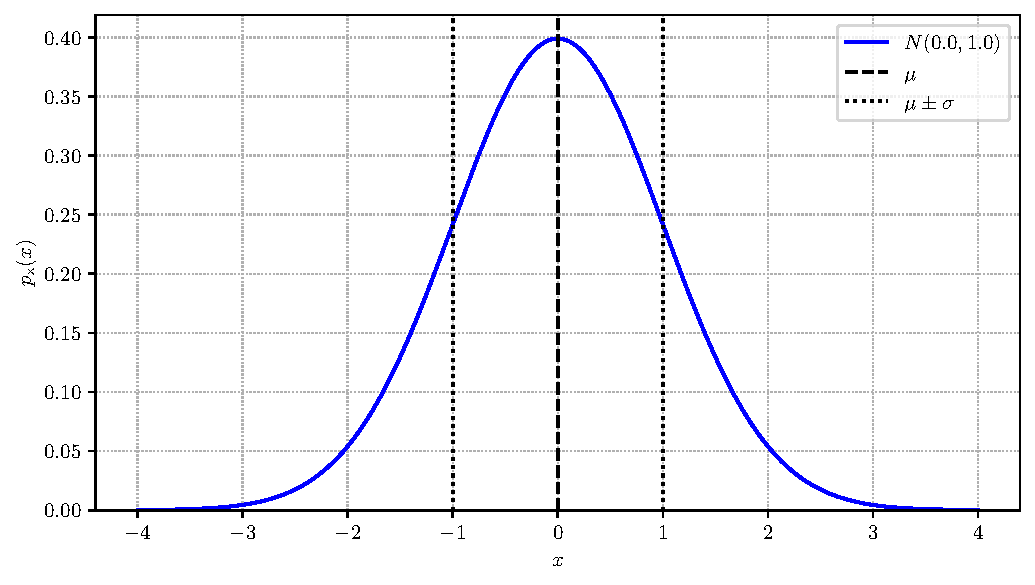
\includegraphics[width=\linewidth]{figs/probability/normal_pdf.pdf} \\
\end{tabular}

\paragraph*{The Poisson Distribution}
The Poisson distribution is a discrete distribution used to model the number of times an event occurs within a fixed interval of time or space. It is the quintessential model for counting rare, independent events happening at a constant average rate, such as the number of emails arriving at a server in one minute, the number of defects per square meter of a material, or the number of radioactive decays in a second. 

The distribution is defined by a single parameter, $\lambda$, which is the average number of events in the given interval. The PMF for the number of observed events, $\mathsf{k}$, is:
\begin{equation}
    p_{\mathsf{k}}(k) = \frac{\lambda^k e^{-\lambda}}{k!} \quad \text{for } k \in \{0, 1, 2, \dots\}
\end{equation}
An important feature of the Poisson distribution is that its mean and variance are equal.

\begin{tabular}{@{}>{\raggedright\arraybackslash}m{0.48\textwidth} >{\raggedleft\arraybackslash}m{0.48\textwidth}@{}}
    \begin{itemize}
        \item \textbf{Notation}: $\mathsf{k} \sim \mathrm{Pois}(\lambda)$
        \item \textbf{Mean}: $\mathbb{E}[\mathsf{k}] = \lambda$
        \item \textbf{Variance}: $\operatorname{Var}(\mathsf{k}) = \lambda$
        \item \textbf{Support}: $\mathsf{k} \in \{0, 1, 2, \dots\} = \mathbb{Z}_{\ge 0}$
    \end{itemize}
    &
    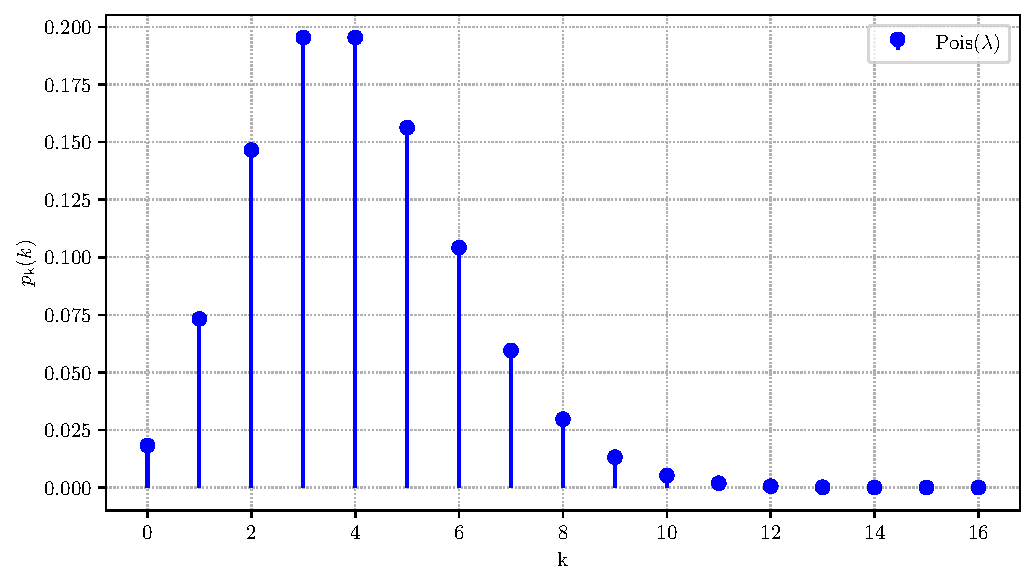
\includegraphics[width=\linewidth]{figs/probability/poisson_pmf.pdf} \\
\end{tabular}

The Poisson distribution can also be viewed as an approximation of the Binomial distribution $B(n, p)$ when the number of trials $n$ is very large and the success probability $p$ is very small, such that $\lambda = np$.

\paragraph*{The Exponential Distribution}
The exponential distribution models the waiting time between events in a Poisson process with constant rate $\lambda$. It is the continuous analog of the geometric distribution and (uniquely among continuous distributions on $[0,\infty)$) has the memoryless property that the probability of an event occurring in the next $t$ units of time is independent of the time already elapsed.

The PDF is
\begin{equation}
    p_{\mathsf{x}}(x) =
    \begin{cases}
        \lambda e^{-\lambda x} & \text{for } x \ge 0 \\[1ex]
        0 & \text{otherwise}
    \end{cases}
\end{equation}

\begin{tabular}{@{}>{\raggedright\arraybackslash}m{0.48\textwidth} >{\raggedleft\arraybackslash}m{0.48\textwidth}@{}}
\begin{itemize}
\item \textbf{Notation}: $\mathsf{x} \sim \mathrm{Exp}(\lambda)$
\item \textbf{Mean}: $\mathbb{E}[\mathsf{x}] = \dfrac{1}{\lambda}$
\item \textbf{Variance}: $\operatorname{Var}(\mathsf{x}) = \dfrac{1}{\lambda^2}$
\item \textbf{Support}: $\mathsf{x} \in [0, \infty) = \mathbb{R}_{\ge 0}$
\end{itemize}
&
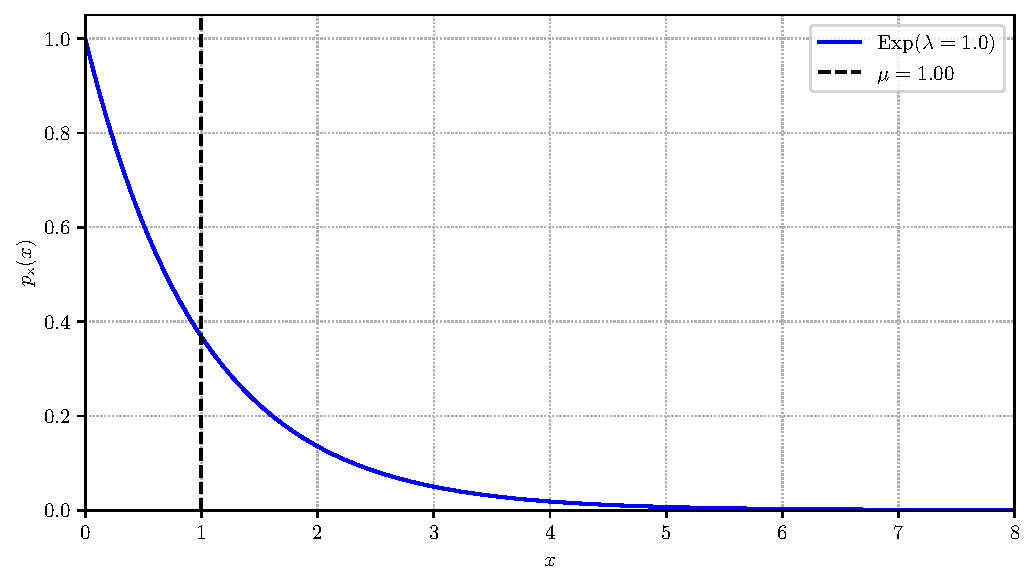
\includegraphics[width=\linewidth]{figs/probability/exponential_pdf.pdf} \\
\end{tabular}

\section{Empirical Distributions}
The probability distributions we have discussed (normal, Poisson, etc.) are theoretical models. They represent a complete and perfect description of a random variable, assuming we know its underlying properties (like $\mu$, $\sigma^2$, or $\lambda$). In any real-world scenario, however, we do not have access to this true, latent distribution. Instead, all we have is a finite collection of data points, or samples, drawn from it. 

The distribution of our collected data is called the \textbf{empirical distribution}. It is our best approximation of the true, underlying distribution. For a discrete random variable, we can define the empirical probability mass function, $\hat{p}_{\mathsf{x}}(x)$\footnote{The hat notation is used universally in statistics to denote an estimator, a value calculated from data that is our best guess for an unknown true value. We'll revisit estimators momentarily.}, as the relative frequency of each outcome in our data:
\begin{equation}
    \hat{p}_{\mathsf{x}}(x) = \frac{\text{number of times } x \text{ was observed}}{\text{total number of samples}} = \frac{N_x}{N}
\end{equation}

\begin{figure}[h!]
    \centering
    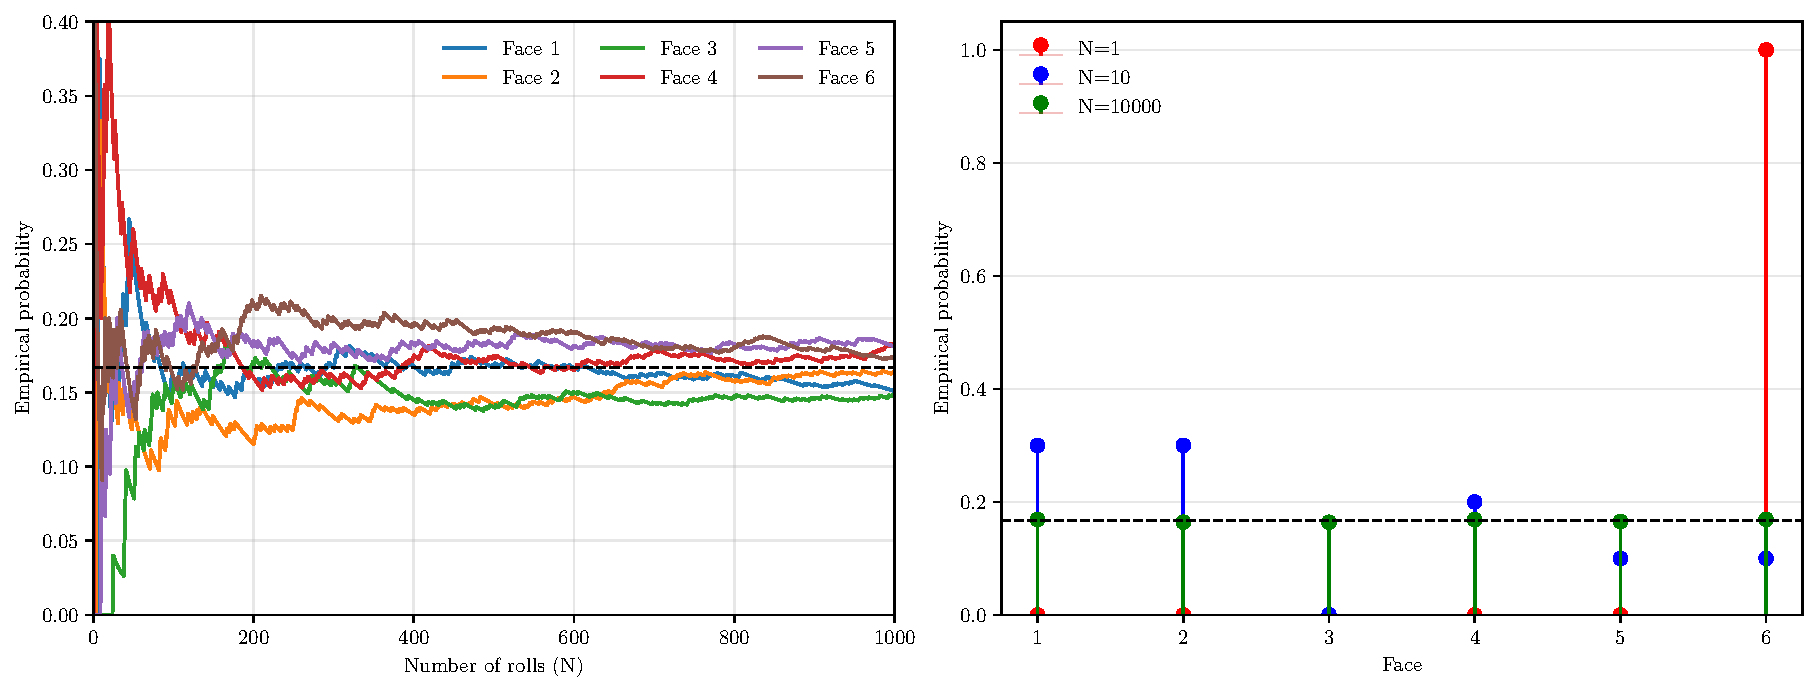
\includegraphics[width=0.98\textwidth]{./figs/probability/empirical_distribution.pdf}
    \caption{Convergence of empirical die-face probabilities (left) and overlaid distribution snapshots at $N=1,10,10000$ (right).}
    \label{fig:die-roll-convergence}
\end{figure}

The \textbf{law of large numbers} guarantees that as our sample size $N$ grows, our empirical distribution will converge to the true underlying distribution. The plot in \autoref{fig:die-roll-convergence} illustrates this perfectly. The left panel traces the running empirical probability of each die face as the number of rolls $N$ increases, with the dashed line at $1/6$ marking the theoretical value. Sampling variability dominates for small $N$ but steadily diminishes. The right panel overlays stem plots of the full discrete distribution at selected sample sizes ($N=1,10,10000$). We can see how a single observation yields an extreme, noisy snapshot, a handful of rolls produces visible imbalance, and a large sample approaches the uniform distribution across faces. The same is true for any underlying and corresponding empirical distribution. If we draw only five samples from a normal distribution, the resulting histogram might look nothing like a bell curve, and any parameters we estimate from it (like the mean) could be very inaccurate. But if we keep adding more samples, we are guaranteed to get a better and better approximation of the true distribution.

\section{The Central Limit Theorem}
We've seen that we use samples from a distribution to learn about it. One of the most common things we compute from a sample is its average. This leads to a question: if we take many different samples and compute the average for each, how will those averages themselves be distributed? The answer is provided by one of the most powerful and perhaps surprising results in all of statistics: the \textbf{central limit theorem (CLT)}.

First, we have to recognize that the sample mean is a random variable itself. If we have a set of $N$ independent and identically distributed (i.i.d.) observations $\{\mathsf{x}_1, \dots, \mathsf{x}_N\}$, their sample mean, $\mathsf{S}_N$, is also a random variable:
\begin{equation}
    \mathsf{S}_N = \frac{1}{N}\sum_{i=1}^N \mathsf{x}_i
\end{equation}
If we were to repeat our experiment (drawing $N$ samples) again, we would get a different value of the sample mean $\mathsf{S}_N$. The CLT describes the distributional shape of this sample mean. Informally, for large $N$, $\mathsf{S}_N$ is approximately normal regardless of the parent distribution's shape (under mild conditions). The formal statement follows.

\begin{definitionBox}
    \textbf{Central Limit Theorem.}
    Let $\{\mathsf{x}_i\}_{i=1}^N$ be i.i.d.\ with mean $\mu$ and finite, nonzero variance $\sigma^2$. Then, as $N\to\infty$,
    \begin{equation}
        \sqrt{N}\,(\mathsf{S}_N-\mu)\ \xrightarrow{d}\ \mathcal{N}(0,\sigma^2),
    \end{equation}
    where $\mathsf{S}_N=\frac{1}{N}\sum_{i=1}^N \mathsf{x}_i$ and $\xrightarrow{d}$ denotes convergence in distribution.
\end{definitionBox}
Equivalently, for large $N$, we have the useful normal approximation
\begin{equation}
    \mathsf{S}_N \approx \mathcal{N}\!\left(\mu,\frac{\sigma^2}{N}\right)  \qquad\text{(large $N$)}
\end{equation}
and, in fact, when the observations are i.i.d.\ with variance $\sigma^2$, the variance identity
\begin{equation}
    \operatorname{Var}(\mathsf{S}_N)=\frac{\sigma^2}{N}
\end{equation}
holds exactly (the normality is the approximation). This tells us two important things:
\begin{enumerate}
    \item The distribution of sample means is centered at the true mean $\mu$.
    \item The variance of the sample means is $\sigma^2/N$. This means that as our sample size $N$ increases, the sample means cluster more and more tightly around the true mean. Our uncertainty in the estimate decreases proportionally to $1/\sqrt{N}$.
\end{enumerate}

\begin{figure}[h!]
    \centering
    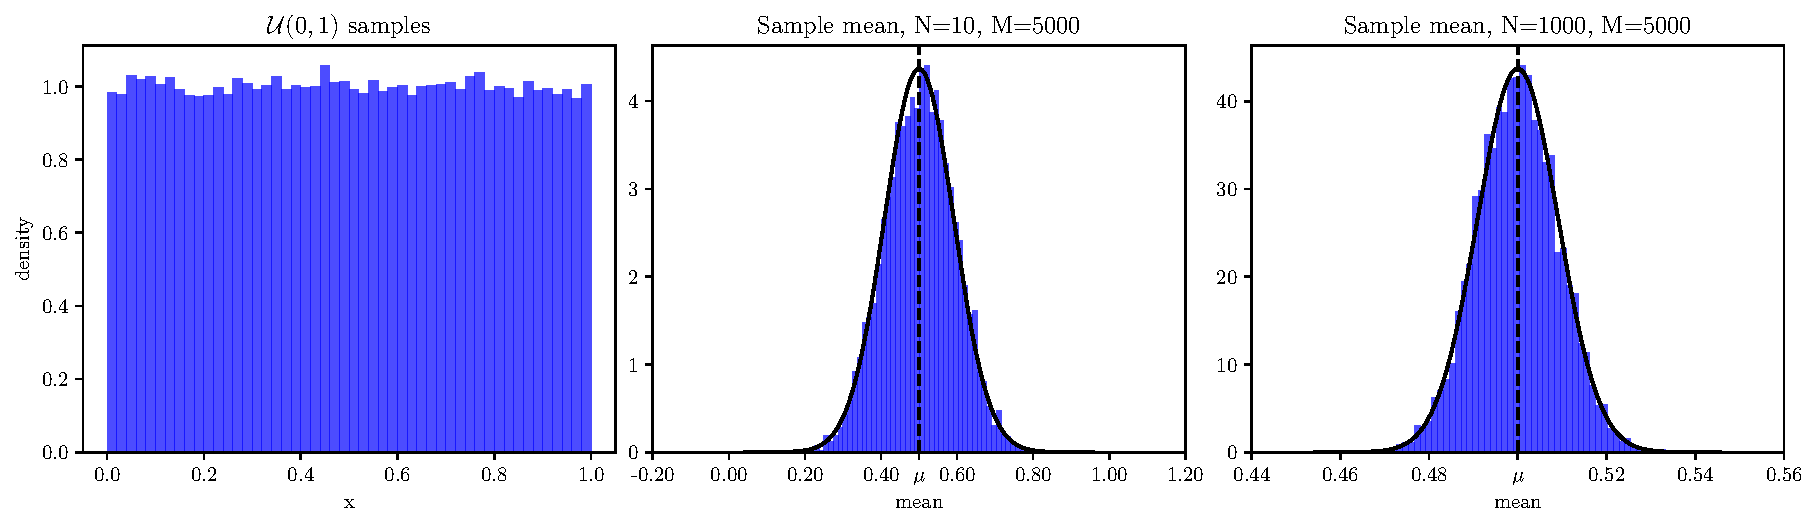
\includegraphics[width=\textwidth]{figs/probability/clt.pdf}
    \caption{Central Limit Theorem demonstration. Left: histogram of raw \(\mathcal{U}(0,1)\) draws. Middle/Right: histograms of the sample mean \(\mathsf{S}_N\) from \(M=5000\) repeated experiments with \(N=10\) and \(N=1000\) per experiment. The solid curve is the normal approximation \(\mathcal{N}(\mu,\sigma^2/N)\) with \(\mu=0.5\) and \(\sigma^2=1/12\); the dashed line marks \(\mu\). As \(N\) increases, the distribution of \(\mathsf{S}_N\) becomes more Gaussian and concentrates around \(\mu\) with standard deviation \(\sigma/\sqrt{N}\). Here, \(M\) is the number of independent repetitions used to build each histogram.}
    \label{fig:clt-demo}
\end{figure}

\begin{warningBox}
    \textbf{Warning: IID required.} The CLT assumes the observations $\{\mathsf{x}_i\}$ are independent and identically distributed with finite variance. If they are dependent or drawn from changing distributions, $\mathsf{S}_N$ may not be approximately $\mathcal{N}(\mu,\sigma^2/N)$ and its variance can be badly misestimated.
    
    As an example of when CLT would not hold, suppose data arrive in identical pairs: $\mathsf{x}_{2k-1}=\mathsf{x}_{2k}$, each pair drawn i.i.d.\ from a distribution with variance $\sigma^2$. Then with the sample mean $\mathsf{S}_N = \frac{1}{N}\sum_{i=1}^N \mathsf{x}_i$, we get
    \begin{equation}
        \operatorname{Var}(\mathsf{S}_N)=\frac{2\sigma^2}{N},
    \end{equation}
    the same as having only $N/2$ independent points. Treating them as i.i.d.\ would give confidence intervals that are too narrow by a factor of $\sqrt{2}$.
\end{warningBox}
    

\section{Estimators and Bias}
The central limit theorem describes the behavior of a specific calculation, the sample mean. This is an example of an \textbf{estimator}: a rule for calculating a value from data to approximate an unknown property of the underlying distribution. We denote estimators using a hat, e.g., the sample mean $\hat{\mu}_{\mathsf{x}} = \mathsf{S}_N$, which we used to estimate the true mean $\mu$. But how do we know if an estimator is a good one? One way is to look at its \textbf{bias}. The bias of an estimator ($\hat{\theta}$) is the difference between its expected value and the true value of the parameter it is trying to estimate ($\theta$):
\begin{equation}
    \text{Bias}(\hat{\theta}) = \mathbb{E}[\hat{\theta}] - \theta
\end{equation}
An estimator is unbiased if its bias is zero, meaning $\mathbb{E}[\hat{\theta}] = \theta$. An unbiased estimator is correct on average, even if any single estimate is off the mark.

\paragraph*{The Sample Mean is Unbiased}
Assume we observe $N$ i.i.d.\ random variables $\{\mathsf{x}_1, \dots, \mathsf{x}_N\}$ drawn from the same distribution $\mathcal{D}$ with population mean $\mu=\mathbb{E}[\mathsf{x}_i]$ and population variance $\sigma^2=\operatorname{Var}(\mathsf{x}_i)$:
\begin{equation}
\mathsf{x}_1,\ldots,\mathsf{x}_N \stackrel{\text{i.i.d.}}{\sim} \mathcal{D}
\label{eq:iid-samples}
\end{equation}
The sample mean is an unbiased estimator of the true mean $\mu$. We can show this easily using the linearity of expectation:
\begin{equation}
    \mathbb{E}[\hat{\mu}_{\mathsf{x}}] = \mathbb{E}\left[\frac{1}{N}\sum_{i=1}^N \mathsf{x}_i\right] = \frac{1}{N}\sum_{i=1}^N \mathbb{E}[\mathsf{x}_i] = \frac{1}{N}\sum_{i=1}^N \mu = \frac{N\mu}{N} = \mu
\end{equation}
Since $\mathbb{E}[\hat{\mu}_{\mathsf{x}}] = \mu$, the bias is zero.

\paragraph*{Estimating Variance and Bessel's Correction}
Now, let's consider estimating the true variance, $\sigma^2$ of the same distribution $\mathcal{D}$ from which $\mathsf{x}_1,\ldots,\mathsf{x}_N$ are drawn as in \autoref{eq:iid-samples}. A natural first guess might be to take the average of the squared differences from our estimated mean:
\begin{equation}
\hat{\sigma}^{2}_{\text{naive}} = \frac{1}{N}\sum_{i=1}^{N}\!\bigl(\mathsf{x}_i-\hat{\mu}_{\mathsf{x}}\bigr)^{2}
\end{equation}
This estimator is biased low. To see this, we first rewrite deviations from the sample mean in terms of deviations from the population mean:
\begin{equation}
    \mathsf{x}_i-\hat{\mu}_{\mathsf{x}} =\bigl(\mathsf{x}_i-\mu\bigr)-\bigl(\hat{\mu}_{\mathsf{x}}-\mu\bigr)
\end{equation}
Next, we expand the square and take expectations (the expectation is over repeated random samples from $\mathcal{D}$):
\begin{align}
    \mathbb{E}\!\left[\hat{\sigma}^{2}_{\text{naive}}\right]
    &=\mathbb{E}\!\left[\frac{1}{N}\sum_{i=1}^{N}\!\bigl((\mathsf{x}_i-\mu)-(\hat{\mu}_{\mathsf{x}}-\mu)\bigr)^{2}\right] \nonumber \\
    &=\mathbb{E}\!\left[\frac{1}{N}\sum_{i=1}^{N}(\mathsf{x}_i-\mu)^{2}\right] -2\,\mathbb{E}\!\left[\frac{1}{N}\sum_{i=1}^{N}(\mathsf{x}_i-\mu)(\hat{\mu}_{\mathsf{x}}-\mu)\right] +\mathbb{E}\!\left[\frac{1}{N}\sum_{i=1}^{N}(\hat{\mu}_{\mathsf{x}}-\mu)^{2}\right]
\end{align}
The first term evaluates to
\begin{equation}
    \frac{1}{N}\sum_{i=1}^{N}\mathbb{E}\!\big[(\mathsf{x}_i-\mu)^{2}\big]=\frac{1}{N}\sum_{i=1}^{N}\sigma^{2}
    =\sigma^{2}
\end{equation}
But $\frac{1}{N}\sum_{i=1}^{N}(\mathsf{x}_i-\mu)=\hat{\mu}_{\mathsf{x}}-\mu$, so the second term becomes
\begin{equation}
    -2\,\mathbb{E}\!\left[(\hat{\mu}_{\mathsf{x}}-\mu)^{2}\right]
    = -2\,\operatorname{Var}(\hat{\mu}_{\mathsf{x}})
\end{equation}
For the third term, the summand does not depend on $i$, so
\begin{equation}
    \mathbb{E}\!\left[\frac{1}{N}\sum_{i=1}^{N}(\hat{\mu}_{\mathsf{x}}-\mu)^{2}\right]
    =\mathbb{E}\!\left[(\hat{\mu}_{\mathsf{x}}-\mu)^{2}\right]
    =\operatorname{Var}(\hat{\mu}_{\mathsf{x}})
\end{equation}
Putting the pieces together, we get
\begin{equation}
    \mathbb{E}\!\left[\hat{\sigma}^{2}_{\text{naive}}\right] 
    = \sigma^2 - 2\,\operatorname{Var}(\hat{\mu}_{\mathsf{x}}) + \operatorname{Var}(\hat{\mu}_{\mathsf{x}})
    =\sigma^{2}-\operatorname{Var}(\hat{\mu}_{\mathsf{x}})
\end{equation}
But for i.i.d.\ data, $\operatorname{Var}(\hat{\mu}_{\mathsf{x}})=\sigma^{2}/N$. Therefore,
\begin{equation}
    \mathbb{E}\!\left[\hat{\sigma}^{2}_{\text{naive}}\right]
    =\left(1-\frac{1}{N}\right)\sigma^{2}
    =\frac{N-1}{N}\,\sigma^{2}
\end{equation}
which shows the bias: the naive estimator systematically underestimates the population variance $\sigma^2$.

It's clear how to remove this bias: just multiply the naive estimator by $N/(N-1)$. We thus define the unbiased sample variance
\begin{equation}
    \hat{\sigma}^{2}_{\text{unbiased}} = \frac{1}{N-1}\sum_{i=1}^{N}\bigl(\mathsf{x}_i-\hat{\mu}_{\mathsf{x}}\bigr)^{2}
\end{equation}
Then, we have
\begin{equation}
    \mathbb{E}[\hat{\sigma}^{2}_{\text{unbiased}}]
    =\frac{N}{N-1}\,\mathbb{E}\!\left[\hat{\sigma}^{2}_{\text{naive}}\right]
    =\frac{N}{N-1}\left(\frac{N-1}{N}\sigma^{2}\right)
    =\sigma^{2}
\end{equation}
so $\hat{\sigma}^{2}_{\text{unbiased}}$ is an unbiased estimator of the population variance $\sigma^{2}$. The intuition here is that the sample mean $\hat{\mu}_{\mathsf{x}}$ is computed from the same sample and ``uses up'' one degree of freedom: once $N-1$ deviations $\mathsf{x}_i-\hat{\mu}_{\mathsf{x}}$ are fixed, the last one must sum to zero. Dividing by $N-1$ instead of $N$ compensates for this constraint and exactly cancels the downward bias. This is known as Bessel's correction.

\begin{exampleBox}
    \textbf{Unbiased Variance Estimator if True Mean is Known}
    What if we know the true mean, $\mu$? Do we still need Bessel's correction? Intuition tells us the answer is no, and the unbiased estimator of the true variance $\sigma^2$ should be
    \begin{equation}
        \tilde{\sigma}^2 = \frac{1}{N}\sum_{i=1}^N \bigl(\mathsf{x}_i - \mu\bigr)^2
    \end{equation}
    Let's check that this is indeed unbiased.
    \begin{equation}
        \mathbb{E}\!\left[\tilde{\sigma}^2\right]
        = \frac{1}{N}\sum_{i=1}^N \mathbb{E}\!\left[(\mathsf{x}_i-\mu)^2\right]
        = \frac{1}{N}\sum_{i=1}^N \operatorname{Var}(\mathsf{x}_i)
        = \sigma^2
    \end{equation}
    Thus, the $N-1$ (Bessel) correction is only needed when $\mu$ is unknown and replaced by the sample mean $\hat{\mu}_{\mathsf{x}}$ computed from the same data.

\end{exampleBox}

\paragraph*{Unbiased \texorpdfstring{$\neq$}{≠} Best MSE} We are foreshadowing a later section a bit here, but this is very important to keep in mind. Unbiasedness concerns the mean of an estimator, not its overall error. The mean-squared error (MSE) decomposes as
\begin{equation}
    \operatorname{MSE}(\hat\theta)
    = \mathbb{E}\!\left[(\hat\theta-\theta)^2\right]
    = \operatorname{Var}(\hat\theta) + \bigl(\operatorname{Bias}(\hat\theta)\bigr)^2
\end{equation}
A slightly biased estimator can have \emph{smaller} MSE if it meaningfully reduces variance. For example, let $\hat\theta$ be unbiased with $\operatorname{Var}(\hat\theta)=\alpha$, and consider another estimator $\tilde\theta$ that just shrinks $\hat\theta$:
\begin{equation}
    \tilde\theta=(1-\lambda)\hat\theta,\qquad 0<\lambda<1
\end{equation}
Then we have
\begin{equation}
    \operatorname{Bias}(\tilde\theta)
    = \mathbb{E}[(1-\lambda)\hat\theta] - \theta
    = (1-\lambda)\mathbb{E}[\hat\theta] - \theta
    = (1-\lambda)\theta - \theta
    = -\lambda\theta
\end{equation}
and
\begin{equation}
    \operatorname{MSE}(\tilde\theta)
    = (1-\lambda)^2 \alpha + \lambda^2 \theta^2
\end{equation}
For sufficiently small $\lambda>0$, we have $\operatorname{MSE}(\tilde\theta) < \operatorname{MSE}(\hat\theta)=\alpha$, so clearly unbiased $\neq$ minimum MSE.


\section{Multivariate Random Variables}
Our discussion so far has focused on single, or univariate, random variables. However, in many engineering and scientific problems, we are interested in multiple random quantities at once. For example, an experiment might measure the temperature and pressure in a reactor, or the velocity of a particle in three dimensions. To handle these cases, we generalize our framework from random variables to random vectors.

\subsection{Random Vectors}
A \textbf{random vector} is simply a vector whose elements are scalar random variables. A random vector $\boldsymbol{\mathsf{x}}$ of dimension $N$ is written as
\begin{equation}
    \boldsymbol{\mathsf{x}} = 
    \begin{bmatrix}
        \mathsf{x}_1 \\
        \mathsf{x}_2 \\
        \vdots \\
        \mathsf{x}_N
    \end{bmatrix}
\end{equation}
For example, the velocity of a particle in 3D space is a random vector $\boldsymbol{\mathsf{v}} = [\mathsf{v}_x, \mathsf{v}_y, \mathsf{v}_z]^\top$. The behavior of a random vector is described by a \textbf{joint probability distribution}. The concepts of CDF and PDF extend directly from the scalar case: the \textbf{joint PDF}, $p_{\boldsymbol{\mathsf{x}}}(\mathbf{x})$, is a function over $\mathbb{R}^N$ that we integrate over a region to find the probability that the vector will fall in that region. Similarly, the \textbf{joint CDF}, $F_{\boldsymbol{\mathsf{x}}}(\mathbf{x})$, is the probability that the vector will fall in a region below $\mathbf{x}$:
\begin{align}
  F_{\boldsymbol{\mathsf{x}}}(\mathbf{x})
  = \mathbb{P}\!\left( \mathsf{x}_1 \le x_1 \,\cap\, \mathsf{x}_2 \le x_2 \,\cap\, \cdots \,\cap\, \mathsf{x}_N \le x_N \right)
\end{align}
If $\boldsymbol{\mathsf{x}}$ has a joint PDF $p_{\boldsymbol{\mathsf{x}}}(\mathbf{x})$, then for any $\mathbf{x}=(x_1,\dots,x_N)$,
\begin{equation}
  F_{\boldsymbol{\mathsf{x}}}(\mathbf{x})
  = \int_{-\infty}^{x_1}\!\cdots\!\int_{-\infty}^{x_N}
      p_{\boldsymbol{\mathsf{x}}}(u_1,\dots,u_N)\,du_1\cdots du_N
\end{equation}
with $p_{\boldsymbol{\mathsf{x}}}(\mathbf{x})\ge 0$ and $\int_{\mathbb{R}^N} p_{\boldsymbol{\mathsf{x}}}(\mathbf{x})\,d\mathbf{x}=1$
For any region $\Omega\subseteq\mathbb{R}^N$,
\begin{equation}
  \mathbb{P}(\boldsymbol{\mathsf{x}}\in\Omega)
  = \int_{\Omega} p_{\boldsymbol{\mathsf{x}}}(\mathbf{x})\,d\mathbf{x}
\end{equation}

The components $\mathsf{x}_1, \dots, \mathsf{x}_N$ are \textbf{independent} if and only if their joint PDF is the product of their individual (marginal) PDFs:
\begin{equation}
    p_{\boldsymbol{\mathsf{x}}}(\mathbf{x}) = \prod_{i=1}^N p_{\mathsf{x}_i}(x_i) \iff \mathsf{x}_1, \dots, \mathsf{x}_N \text{ are independent}
\end{equation}

The mean of a random vector is a vector containing the means of each of its components:
\begin{equation}
    \boldsymbol{\mu}_{\boldsymbol{\mathsf{x}}} = \mathbb{E}[\boldsymbol{\mathsf{x}}] = \langle \boldsymbol{\mathsf{x}} \rangle = 
\begin{bmatrix}
    \mathbb{E}[\mathsf{x}_1] \\
    \mathbb{E}[\mathsf{x}_2] \\
    \vdots \\
    \mathbb{E}[\mathsf{x}_N]
\end{bmatrix}
\end{equation}

\begin{exampleBox}
    \textbf{Example (Bivariate PDF as a Product of Marginals):}
    We take two \emph{independent} scalar random variables:
    \begin{equation}
    \mathsf{x}\sim\mathcal{N}(0,1),\qquad
    \mathsf{y}\sim\mathcal{N}(0,4)
    \end{equation}
    with independence meaning $p_{\mathsf{x},\mathsf{y}}(x,y)=p_{\mathsf{x}}(x)\,p_{\mathsf{y}}(y)$. The marginal PDFs are
    \begin{equation}
    p_{\mathsf{x}}(x)=\frac{1}{\sqrt{2\pi}}\exp\!\Big(-\frac{x^{2}}{2}\Big),
    \qquad
    p_{\mathsf{y}}(y)=\frac{1}{\sqrt{2\pi}\cdot 2}\exp\!\Big(-\frac{y^{2}}{8}\Big)
    \end{equation}
    So the joint PDF is the simple product
    \begin{equation}
        p_{\mathsf{x},\mathsf{y}}(x,y)
        = p_{\mathsf{x}}(x)\,p_{\mathsf{y}}(y)
        = \frac{1}{2\pi\cdot 2}\,
        \exp\!\Big(-\frac{x^{2}}{2}-\frac{y^{2}}{8}\Big)
    \end{equation}
    The density is shown in \autoref{fig:bivariate-gaussian-independent}.
    \begin{figure}[H]
        \centering
        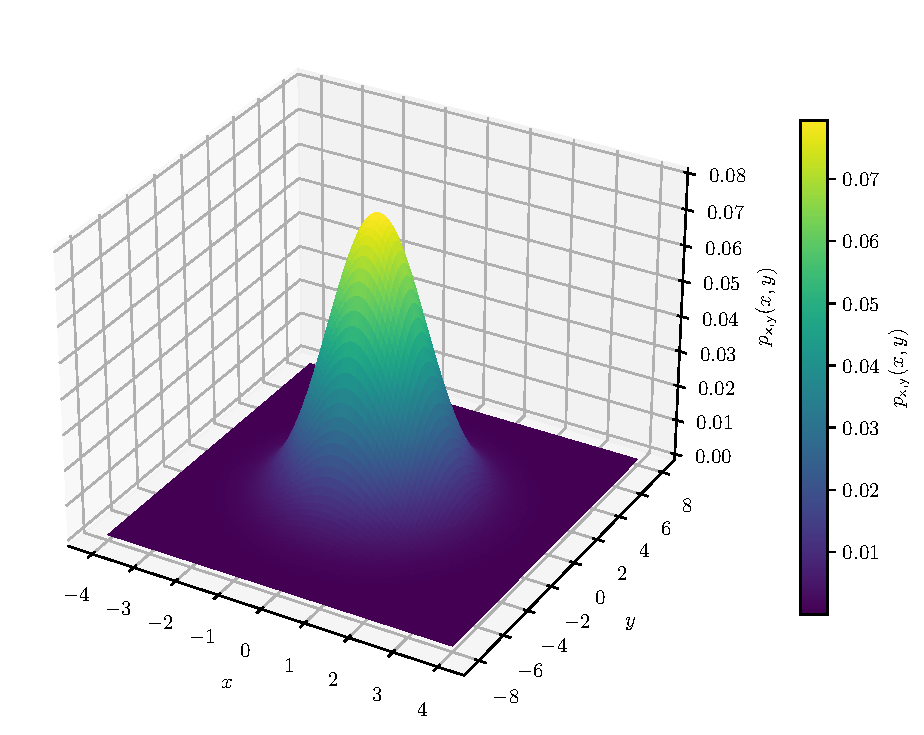
\includegraphics[width=.5\textwidth]{figs/probability/bivariate_gaussian_independent.pdf}
        \caption{Bivariate Gaussian density with independent components.}
        \label{fig:bivariate-gaussian-independent}
    \end{figure}
\end{exampleBox}

\section{Covariance and Correlation}
While the mean vector describes the central tendency of each component, it tells us nothing about the relationships \textit{between} the components. Do they tend to increase together? Or does one tend to decrease when the other increases? This is measured by the \textbf{covariance}.

The covariance between two scalar random variables $\mathsf{x}_i$ and $\mathsf{x}_j$ is the expected product of their deviations from their respective means $\mu_i$ and $\mu_j$:
\begin{equation}
    \operatorname{Cov}(\mathsf{x}_i, \mathsf{x}_j) = \mathbb{E}\big[(\mathsf{x}_i - \mu_i)(\mathsf{x}_j - \mu_j)\big] = \mathbb{E}[\mathsf{x}_i \mathsf{x}_j] - \mu_i \mu_j
\end{equation}
The sign of the covariance tells us the nature of the linear relationship:
\begin{itemize}
    \item $\operatorname{Cov}(\mathsf{x}_i, \mathsf{x}_j) > 0$: $\mathsf{x}_i$ and $\mathsf{x}_j$ tend to be on the same side of their means. They have a positive linear relationship.
    \item $\operatorname{Cov}(\mathsf{x}_i, \mathsf{x}_j) < 0$: $\mathsf{x}_i$ and $\mathsf{x}_j$ tend to be on opposite sides of their means. They have a negative linear relationship.
    \item $\operatorname{Cov}(\mathsf{x}_i, \mathsf{x}_j) = 0$: There is no linear relationship between them. They are said to be uncorrelated.
\end{itemize}

For a random vector $\boldsymbol{\mathsf{x}}$, we summarize all of these pairwise relationships in the \textbf{covariance matrix} $\mathbf{C}$. The element $C_{ij}$ is the covariance between $\mathsf{x}_i$ and $\mathsf{x}_j$.
\begin{equation}
    \mathbf{C} = \begin{bmatrix}
        \operatorname{Var}(\mathsf{x}_1) & \operatorname{Cov}(\mathsf{x}_1, \mathsf{x}_2) & \cdots & \operatorname{Cov}(\mathsf{x}_1, \mathsf{x}_N) \\
        \operatorname{Cov}(\mathsf{x}_2, \mathsf{x}_1) & \operatorname{Var}(\mathsf{x}_2) & \cdots & \operatorname{Cov}(\mathsf{x}_2, \mathsf{x}_N) \\
        \vdots & \vdots & \ddots & \vdots \\
        \operatorname{Cov}(\mathsf{x}_N, \mathsf{x}_1) & \operatorname{Cov}(\mathsf{x}_N, \mathsf{x}_2) & \cdots & \operatorname{Var}(\mathsf{x}_N)
    \end{bmatrix}
\end{equation}
The diagonal entries of the covariance matrix are the variances of each component, $C_{ii} = \operatorname{Cov}(\mathsf{x}_i, \mathsf{x}_i) = \operatorname{Var}(\mathsf{x}_i)$, and the off-diagonal entries describe how the components co-vary. If the off-diagonal entries are all zero, the covariance matrix is diagonal, and the components are said to be pairwise uncorrelated.

\begin{exampleBox}
    \textbf{Example (Covariance and Scatter Patterns):}
    Consider three zero-mean bivariate normal random vectors
    \(
    \boldsymbol{\mathsf{x}}^{(k)}\sim \mathcal{N}(\mathbf{0},\,\mathbf{\Sigma}^{(k)})
    \)
    with covariance matrices
    \[
    \mathbf{\Sigma}^{(1)}=\begin{bmatrix}1&0\\0&1\end{bmatrix},\quad
    \mathbf{\Sigma}^{(2)}=\begin{bmatrix}1&0.8\\0.8&1\end{bmatrix},\quad
    \mathbf{\Sigma}^{(3)}=\begin{bmatrix}1&-0.8\\-0.8&1\end{bmatrix}.
    \]
    A major point here is that for the cases with off-diagonal entries, we do \emph{not} have the product of the marginal PDFs as the joint PDF. Instead, the joint PDF has the following quadratic-exponential form (for 10.34, don't worry about knowing where this comes from, but it is a general result for multivariate Gaussians):
    \begin{equation}
    p_{\boldsymbol{\mathsf{x}}^{(k)}}(\mathbf{x})
    = \frac{1}{2\pi\sqrt{\det\mathbf{\Sigma}^{(k)}}}\,
    \exp\!\left(
    -\frac{1}{2}\,\mathbf{x}^\top \left(\mathbf{\Sigma}^{(k)}\right)^{-1}\mathbf{x}
    \right),\qquad \mathbf{x}=[x_1,x_2]^\top
    \end{equation}
    We draw i.i.d.\ samples from each $p_{\boldsymbol{\mathsf{x}}^{(k)}}(\mathbf{x})$ and plot them:
    \begin{center}
      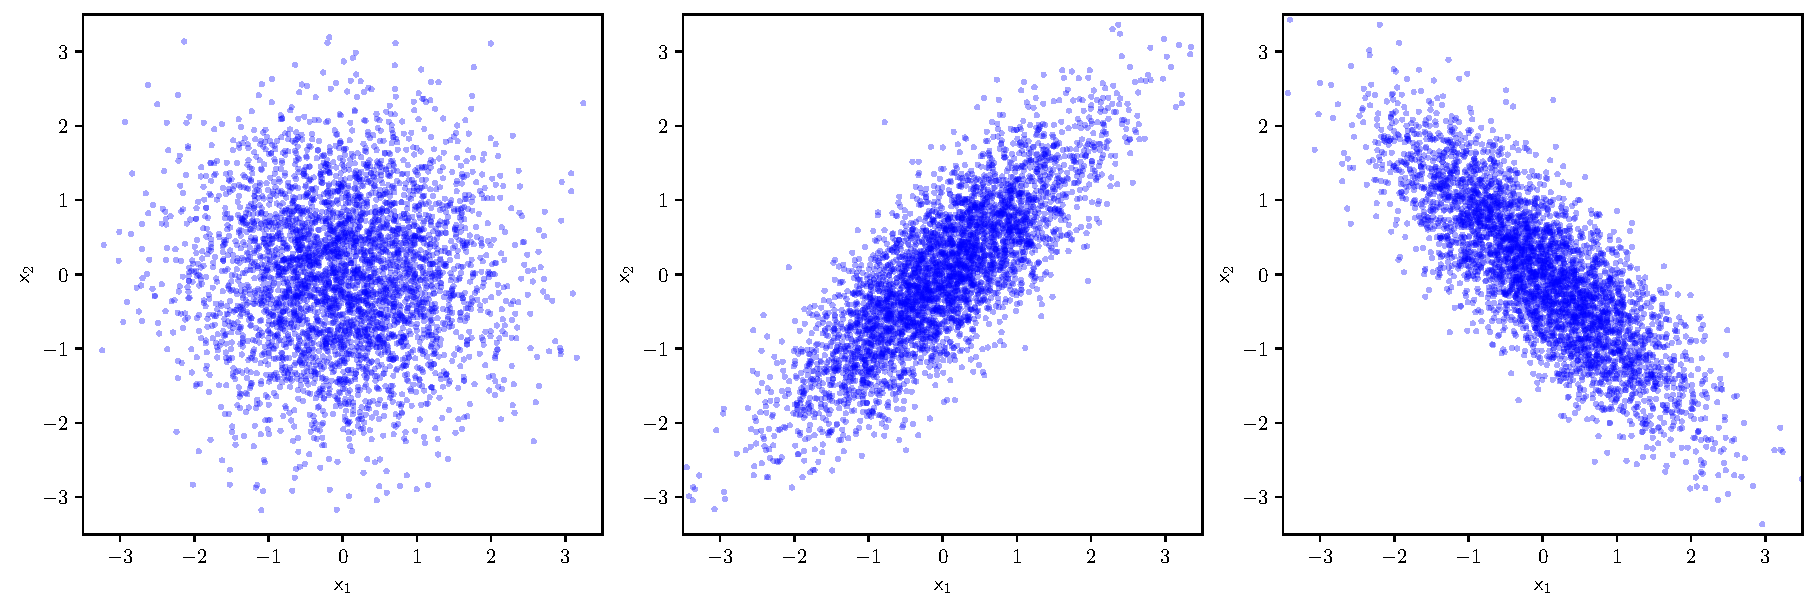
\includegraphics[width=\textwidth]{figs/probability/covariance_panels.pdf}
    \end{center}
    \textit{Interpretation.} 
    $\mathbf{\Sigma}^{(1)}$ is diagonal (uncorrelated); the cloud is circular/axis-aligned. 
    $\mathbf{\Sigma}^{(2)}$ has positive off-diagonals; the cloud tilts upward (positive linear relationship).
    $\mathbf{\Sigma}^{(3)}$ has negative off-diagonals; the cloud tilts downward (negative linear relationship).
\end{exampleBox}
    

\paragraph*{Independence vs.\ Uncorrelatedness}
The relationship between independence and correlation is a common point of confusion. The rule is simple: independence implies uncorrelatedness, but uncorrelatedness does not imply independence. Pondering upon this a bit, it is clear why. If two random variables are independent, their covariance is zero by definition, so they must be uncorrelated also by definition. However, if all we know is that the covariance is zero, this only means that there is no \emph{linear} relationship between the two. A strong nonlinear relationship can still exist, as shown in \autoref{fig:uncorrelated-dependent}.\footnote{We note that for the special case of jointly Gaussian variables, zero covariance \emph{does} imply independence.}

\begin{exampleBox}
    \textbf{Example (Uncorrelated but Dependent).}
    Let $\mathsf{x}_1 \sim \mathcal{N}(0,1)$ and let $\varepsilon$ be independent noise with $\mathbb{E}[\varepsilon]=0$.
    Define
    \begin{equation}
    \mathsf{x}_2 = \mathsf{x}_1^2 + \varepsilon
    \end{equation}
    Then $\mathbb{E}[\mathsf{x}_1]=0$ and $\mathbb{E}[\mathsf{x}_1^3]=0$ (symmetry), so
    \begin{equation}
    \mathrm{Cov}(\mathsf{x}_1,\mathsf{x}_2)
    = \mathrm{Cov}(\mathsf{x}_1,\mathsf{x}_1^2) + \mathrm{Cov}(\mathsf{x}_1,\varepsilon)
    = \mathbb{E}[\mathsf{x}_1^3] - \mathbb{E}[\mathsf{x}_1]\mathbb{E}[\mathsf{x}_1^2] + 0
    = 0
    \end{equation}
    Thus the variables are \emph{uncorrelated}. However, $\mathsf{x}_2$ is (almost) a deterministic function of $\mathsf{x}_1$, so they are clearly \emph{dependent}. The scatter below shows the strong nonlinear relation without any linear trend:
    \begin{figure}[H]
        \centering
        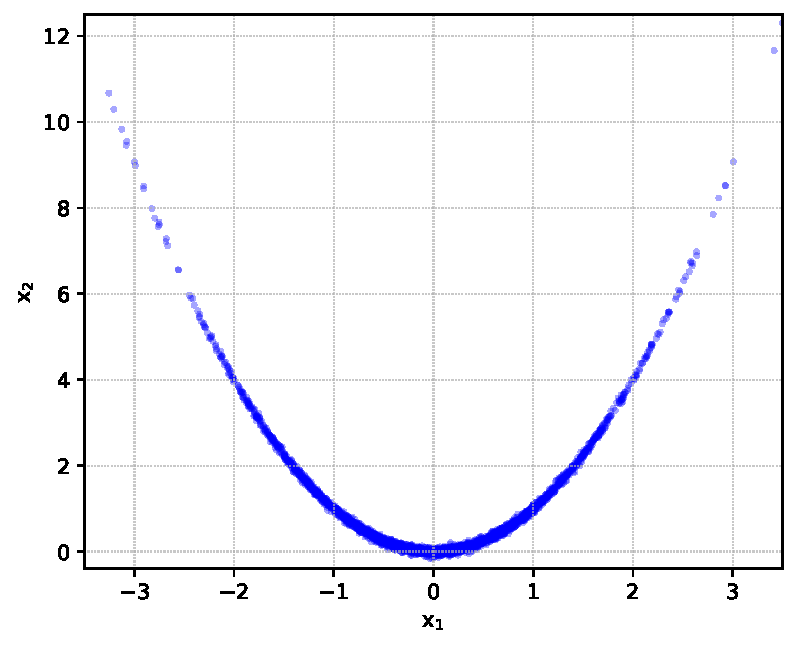
\includegraphics[width=.4\textwidth]{figs/probability/uncorrelated_dependent.pdf}
        \caption{Uncorrelated but dependent.}
        \label{fig:uncorrelated-dependent}
    \end{figure}
\end{exampleBox}

Finally, since the magnitude of covariance depends on the units of the variables, it is often normalized into a dimensionless quantity called the Pearson correlation coefficient, $r$. The square of this value, the \textbf{coefficient of determination} $r^2$, measures the proportion of the variance in one variable that is predictable from the other variable:
\begin{equation}
    r^2(\mathsf{x}, \mathsf{y}) 
    = \left(\frac{\operatorname{Cov}(\mathsf{x}, \mathsf{y})}{\sigma_{\mathsf{x}}\sigma_{\mathsf{y}}}\right)^2
    = \frac{\left(\mathbb{E}[\mathsf{x}\mathsf{y}] - \mathbb{E}[\mathsf{x}]\mathbb{E}[\mathsf{y}]\right)^2}{\left(\mathbb{E}[\mathsf{x}^2] - \mathbb{E}[\mathsf{x}]^2\right)\left(\mathbb{E}[\mathsf{y}^2] - \mathbb{E}[\mathsf{y}]^2\right)}
\end{equation}
To visualize this, we simulate three bivariate normals, plot the scatter, and overlay the least-squares line.
\begin{center}
  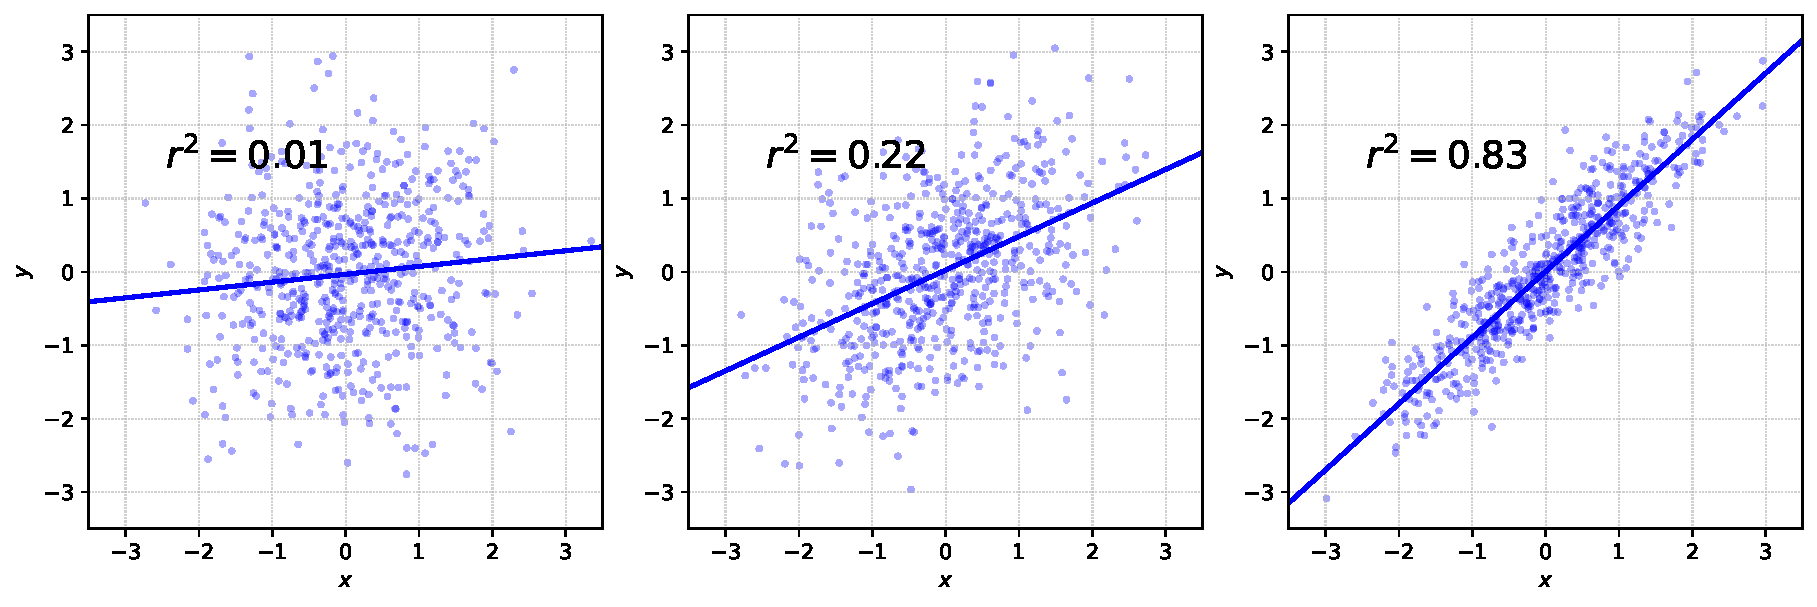
\includegraphics[width=\textwidth]{figs/probability/r2_panels.pdf}
\end{center}

\subsection{Conditional Probability}
We have seen how a joint PDF $p_{\mathbf{\mathsf{x}}}(\mathbf{x})$ describes the behavior of a random vector. But how does our knowledge about one component of the vector change once we observe the value of another? This is the domain of \textbf{conditional probability distributions}. The conditional PDF of $\mathsf{x}_2$ given that we have observed $\mathsf{x}_1=x_1$ is defined as the joint PDF divided by the marginal PDF of the known variable:
\begin{equation}
    p_{\mathsf{x}_2 \mid \mathsf{x}_1}(x_2 \mid x_1) = \frac{p_{\mathsf{x}_1, \mathsf{x}_2}(x_1, x_2)}{p_{\mathsf{x}_1}(x_1)} \quad \text{provided } p_{\mathsf{x}_1}(x_1) > 0
\end{equation}
Intuitively, you can think of the joint PDF as a mountain range over the $(x_1, x_2)$ plane. Observing that $\mathsf{x}_1=x_1$ is like taking a vertical slice of that mountain at a specific $x_1$ value. The curve you see on that slice is the shape of the conditional distribution. We divide by $p_{\mathsf{x}_1}(x_1)$ to re-normalize the area under this curve to 1, making it a valid PDF.

By rearranging this definition, we get the \textbf{chain rule of probability} for random variables, which allows us to build a joint distribution from conditional and marginal parts:
\begin{equation}
    p_{\mathsf{x}_1, \mathsf{x}_2}(x_1, x_2) = p_{\mathsf{x}_2 \mid \mathsf{x}_1}(x_2 \mid x_1)p_{\mathsf{x}_1}(x_1)
\end{equation}

\begin{exampleBox}
    \textbf{Example}: Consider a 2D random vector where $\mathsf{x}_1 \sim \mathcal{N}(0, 0.25)$ and the conditional distribution of $\mathsf{x}_2$ is given by $\mathsf{x}_2 \mid \mathsf{x}_1 \sim \mathcal{N}(-2x_1, 1)$. How does the distribution of $\mathsf{x}_2$ change for different observations of $\mathsf{x}_1$?
    \begin{itemize}
        \item If we observe $x_1 = 0$, the distribution of $\mathsf{x}_2$ is $\mathcal{N}(-2(0), 1) = \mathcal{N}(0, 1)$.
        \item If we observe $x_1 = 1$, the distribution of $\mathsf{x}_2$ becomes $\mathcal{N}(-2(1), 1) = \mathcal{N}(-2, 1)$.
    \end{itemize}
    Our knowledge of $\mathsf{x}_1$ directly influences our expectation of $\mathsf{x}_2$. This is visualized in \autoref{fig:conditional-slice}, where the conditional distribution is a vertical slice of the joint distribution.
\end{exampleBox}

\begin{figure}[h!]
    \centering
    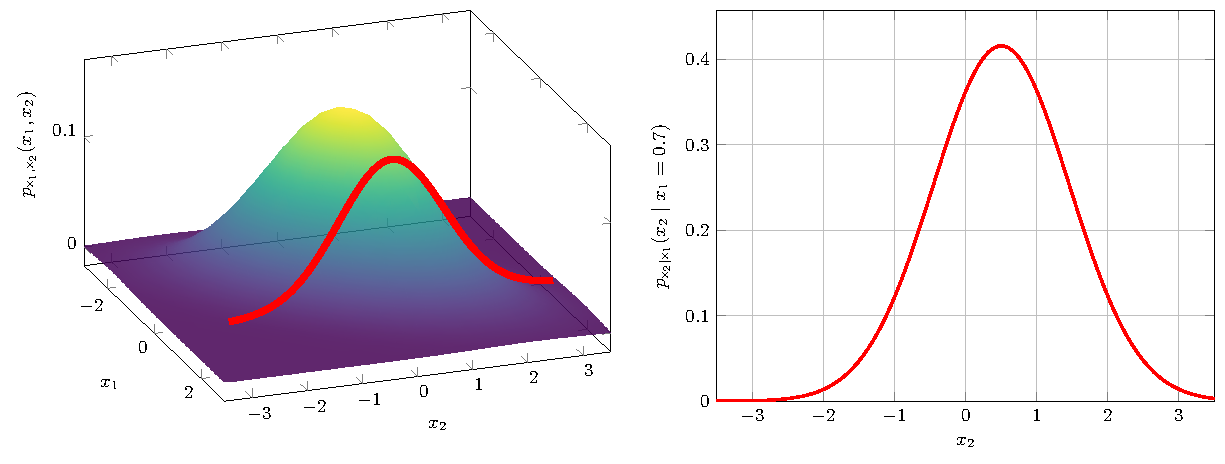
\includegraphics[width=0.8\textwidth]{figs/probability/conditional_fig.pdf}
    \caption{A visualization of conditional probability. The blue scatter plot represents samples from a joint distribution. Fixing a value of $\mathsf{x}_1$ (e.g., $x_1=0$ or $x_1=1$) is like taking a vertical slice. The distribution of the points within that slice is the conditional distribution of $\mathsf{x}_2$ given $\mathsf{x}_1$.}
    \label{fig:conditional-slice}
\end{figure}

\paragraph*{Conditional Independence}
A related concept is conditional independence. Two random variables $\mathsf{x}_1$ and $\mathsf{x}_2$ are conditionally independent given a third variable $\mathsf{x}_3$ if, once we know $\mathsf{x}_3$, knowing $\mathsf{x}_1$ gives us no additional information about $\mathsf{x}_2$. Mathematically:
\begin{equation}
    p(x_1, x_2 \mid x_3) = p(x_1 \mid x_3)p(x_2 \mid x_3)
\end{equation}
For example, two noisy temperature sensors are not independent; if one reads high, the other likely will too. But they are \textit{conditionally independent given the true temperature}. Once we know the true temperature, the noise in one sensor reading is independent of the noise in the other.

\subsection{Marginalization}
Often, we have a high-dimensional joint distribution but are only interested in the distribution of a single component. How do we get the PDF of $\mathsf{x}_1$ alone from $p_{\mathsf{x}_1, \mathsf{x}_2}(x_1, x_2)$? The process is called \textbf{marginalization}. To find the marginal distribution of one variable, we ``integrate out'' all other variables. This is the continuous version of the law of total probability.
\begin{equation}
    p_{\mathsf{x}_1}(x_1) = \int_{-\infty}^{\infty} p_{\mathsf{x}_1, \mathsf{x}_2}(x_1, x_2)\,dx_2
\end{equation}
We can substitute the chain rule into this expression to see the connection to conditioning:
\begin{equation}
    p_{\mathsf{x}_1}(x_1) = \int_{-\infty}^{\infty} p_{\mathsf{x}_1 \mid \mathsf{x}_2}(x_1 \mid x_2)p_{\mathsf{x}_2}(x_2)\,dx_2
\end{equation}
Visually, marginalization is like taking the 3D mountain of the joint PDF and projecting or collapsing its mass onto one of the axes. The resulting shadow on that axis is the marginal PDF.

\begin{figure}[h!]
    \centering
    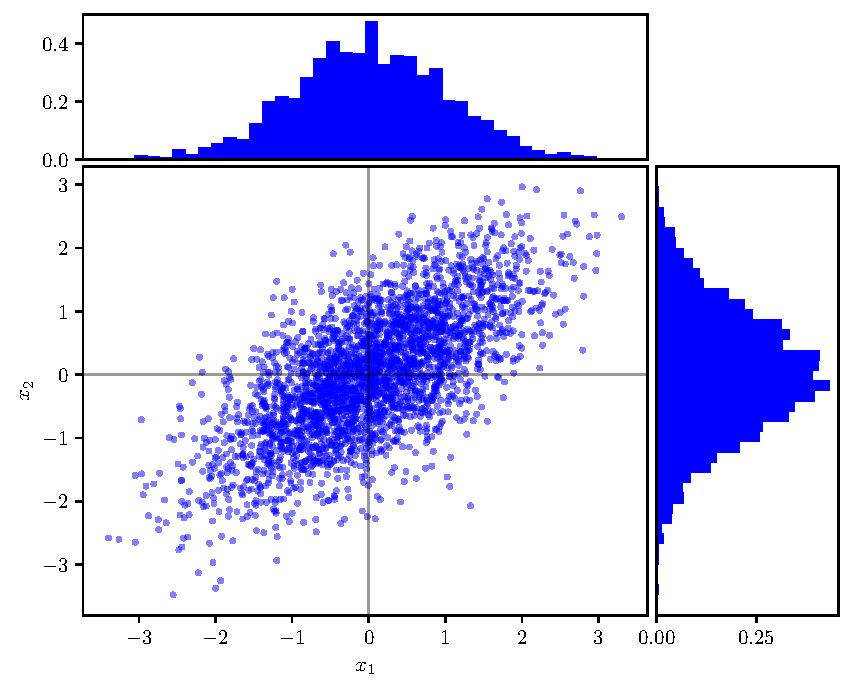
\includegraphics[width=0.7\textwidth]{figs/probability/marginalization.pdf}
    \caption{A scatter plot with marginal distributions shown as histograms. The central scatter plot shows samples from the joint distribution $p_{\mathsf{x}_1, \mathsf{x}_2}(x_1, x_2)$. The histograms on the margins (bottom and left) show the marginal distributions $p_{\mathsf{x}_1}(x_1)$ and $p_{\mathsf{x}_2}(x_2)$, obtained by projecting the joint data onto each axis.}
    \label{fig:marginalization}
\end{figure}

% MC: maybe (B) and (C) are confusing here, but good to expose students to this way of thinking?
\begin{exampleBox}
    \textbf{Example (Marginalizing a PDF in Several Equivalent Ways).}
    Suppose we build a 2D random vector by using the following:
    \begin{equation}
        \mathsf{x}_1 \sim \mathcal{N}(0,\;0.25), 
        \qquad 
        \mathsf{x}_2 \mid \mathsf{x}_1=x_1 \sim \mathcal{N}(-2x_1,1)
    \end{equation}
    with $\mathsf{x}_1$ and the conditional noise independent. The joint PDF is
    \begin{equation}
        p_{\mathsf{x}_1,\mathsf{x}_2}(x_1,x_2)
        = p_{\mathsf{x}_2\mid \mathsf{x}_1}(x_2\mid x_1)\,p_{\mathsf{x}_1}(x_1)
    \end{equation}
    
    We are interested in the marginal PDF of $\mathsf{x}_2$, i.e., $p_{\mathsf{x}_2}(x_2)$. Let's look at a few ways we can do this.
    
    \medskip
    \textit{(A) By definition: integrate out the unneeded variable.}
    \begin{align}
    p_{\mathsf{x}_2}(x_2)
    &= \int_{-\infty}^{\infty} p_{\mathsf{x}_1,\mathsf{x}_2}(x_1,x_2)\,dx_1 \\
    &= \int_{-\infty}^{\infty} p_{\mathsf{x}_2\mid \mathsf{x}_1}(x_2\mid x_1)\,p_{\mathsf{x}_1}(x_1)\,dx_1 \label{eq:marg_def} \\
    &= \int_{-\infty}^{\infty}
    \frac{1}{\sqrt{2\pi}}\exp\!\left(-\frac{(x_2+2x_1)^2}{2}\right)\;
    \frac{1}{\sqrt{2\pi\cdot 0.25}}\exp\!\left(-\frac{x_1^2}{2\cdot 0.25}\right)\,dx_1
    \end{align}
    This integral is a convolution of Gaussians in $x_1$. Completing the square (or using a standard identity) gives
    \begin{equation}
        p_{\mathsf{x}_2}(x_2)=\mathcal{N}\big(0,1+4\cdot 0.25\big)=\mathcal{N}(0,2)
    \end{equation}
    
    \medskip
    \textit{(B) Using moments.}
    This is a quicker way to do it. We know that the marginal distribution of $\mathsf{x}_2$ is Gaussian (a linear combination of independent Gaussians is Gaussian), so we can completely characterize it by its mean and variance, which are easily computed using the information we have. From the model, $\mathbb{E}[\mathsf{x}_2\mid \mathsf{x}_1]= -2\mathsf{x}_1$ and $\operatorname{Var}(\mathsf{x}_2\mid \mathsf{x}_1)=1$. The law of total expectation/variance\footnote{We don't cover the latter in 10.34, so you would not be expected to use this route on an exam. But we provide this route for illustration purposes.} gives
    \begin{gather}
        \mathbb{E}[\mathsf{x}_2]=\mathbb{E}\!\big[\mathbb{E}[\mathsf{x}_2\mid \mathsf{x}_1]\big]
        =-2\,\mathbb{E}[\mathsf{x}_1]=0, \\
        \operatorname{Var}(\mathsf{x}_2)=\mathbb{E}\!\big[\operatorname{Var}(\mathsf{x}_2\mid \mathsf{x}_1)\big]
        +\operatorname{Var}\!\big(\mathbb{E}[\mathsf{x}_2\mid \mathsf{x}_1]\big)
        =1+4\,\operatorname{Var}(\mathsf{x}_1)=1+4(0.25)=2
    \end{gather}
    Therefore, $\mathsf{x}_2\sim\mathcal{N}(0,2)$.
    
    \medskip
    \textit{(C) Linear-Gaussian viewpoint.} Even quicker! We equivalently write $\mathsf{x}_2=-2\mathsf{x}_1+\varepsilon$ with $\varepsilon\sim\mathcal{N}(0,1)$ independent of $\mathsf{x}_1$. Then immediately we have
    \begin{equation}
        \mathsf{x}_2 \sim \mathcal{N}\!\big(-2\cdot 0,(-2)^2\cdot 0.25 + 1\big)=\mathcal{N}(0,2)
    \end{equation}
    Note that we are relying on the linearity and Gaussianity of the distribution to do this.
\end{exampleBox}

\section{A Unified View of Probability Distributions}

This chapter has introduced several probability distributions as separate entities, but it is important to recognize that they exist within a deeply interconnected web. Indeed, many distributions can be seen as special cases, generalizations, or limiting transformations of others. A classic example of this is the relationship between the Bernoulli, binomial, and normal distributions.

\paragraph*{Bernoulli to Binomial:} A single coin flip, with a binary outcome (e.g., success or failure), is a Bernoulli trial. The probability of success, $p$, is the only parameter. If you perform $n$ independent and identical Bernoulli trials and count the total number of successes, this count follows a binomial distribution. Thus, a binomial random variable is simply the sum of $n$ independent Bernoulli random variables.
    
\paragraph*{Binomial to Normal:} The central limit theorem states that the sum of a large number of independent and identically distributed random variables will be approximately normally distributed. As a result, when the number of trials $n$ becomes large, the shape of the discrete binomial distribution becomes so close to the continuous normal distribution that the normal can be used as an excellent approximation for the binomial.

These connections are illustrative, not exhaustive. Many further bridges exist: the rare-event limit links binomial to Poisson; Poisson processes connect counts to exponential and gamma waiting times; the normal, $\chi^2$, $t$, and $F$ families arise from sums and ratios; conjugate mixtures (e.g., beta-binomial, Dirichlet-multinomial) tie priors to likelihoods; monotonic transformations give rise to new laws (e.g., lognormal from a normal); and multivariate generalizations introduce structures such as the Wishart distribution (a generalization of the gamma distribution). A great resource for a comprehensive overview of the relationships between univariate distributions is \href{https://www.math.wm.edu/~leemis/chart/UDR/UDR.html}{this beautiful interactive chart} produced by Prof.\ Larry Leemis at William \& Mary.

\subsection{Convolution}
The relationship we just discussed, where a binomial random variable is the sum of independent Bernoulli random variables, is a specific case of a more general concept called convolution. Convolution is the mathematical operation that gives the probability distribution of a sum of two independent random variables.

Suppose we have two independent random variables, $\mathsf{x}$ and $\mathsf{y}$. We are interested in the distribution of their sum, $\mathsf{s} = \mathsf{x} + \mathsf{y}$. To find the probability of a specific total outcome $\mathsf{s}$, we must consider every possible pair of outcomes, one from $\mathsf{x}$ and one from $\mathsf{y}$, that sum to $\mathsf{s}$. Because $\mathsf{x}$ and $\mathsf{y}$ are independent, the probability of each such pair is the product of their individual probabilities. We then add up the probabilities of all these possible pairs to get the total probability for $\mathsf{s}$. This process of pairing up, multiplying, and summing is precisely what convolution represents.

\paragraph*{The Discrete Case}
Let $\mathsf{x}$ and $\mathsf{y}$ be independent, integer-valued random variables with PMFs $p_{\mathsf{x}}$ and $p_{\mathsf{y}}$, respectively. The PMF of their sum, $\mathsf{s} = \mathsf{x} + \mathsf{y}$, is given by the discrete convolution of $p_{\mathsf{x}}$ and $p_{\mathsf{y}}$, denoted $(p_{\mathsf{x}} * p_{\mathsf{y}})(s)$:
\begin{equation}
    p_{\mathsf{s}}(s) = (p_{\mathsf{x}} * p_{\mathsf{y}})(s) = \sum_{x} p_{\mathsf{x}}(x) \cdot p_{\mathsf{y}}(s-x)
\end{equation}
The sum is over all possible values $x$ in the support of $\mathsf{x}$. For each $x$, the corresponding value from $\mathsf{y}$ that would result in the sum $s$ is $s-x$.

\begin{exampleBox}
    \textbf{Example: Deriving the Discrete Convolution Formula}

    Our goal is to find the probability that the sum $\mathsf{s} = \mathsf{x} + \mathsf{y}$ equals some specific value $s$. The event ``the sum is $s$'' can happen in many mutually exclusive ways. For every possible value $x$ that the random variable $\mathsf{x}$ can take, the event occurs if $\mathsf{y}$ takes the value $s-x$. We can write the total event as a union of these disjoint sub-events:
    \begin{equation}
        \{\mathsf{s} = s\} = \bigcup_{x} \{\mathsf{x}=x \text{ and } \mathsf{y}=s-x\}
    \end{equation}
    For example, if we're rolling two dice and want a total of 4, the event is $\{\text{die 1}=1, \text{die 2}=3\} \cup \{\text{die 1}=2, \text{die 2}=2\} \cup \{\text{die 1}=3, \text{die 2}=1\}$. Because these ways are mutually exclusive ($\mathsf{x}$ cannot be both 1 and 2 at the same time), the probability of the total event is the sum of the probabilities of the sub-events:
    \begin{equation}
        P(\mathsf{s}=s) = \sum_{x} P(\mathsf{x}=x \text{ and } \mathsf{y}=s-x)
    \end{equation}
    Now, we use our key assumption that $\mathsf{x}$ and $\mathsf{y}$ are independent. The probability of two independent events both occurring is the product of their individual probabilities:
    \begin{equation}
        P(\mathsf{x}=x \text{ and } \mathsf{y}=s-x) = P(\mathsf{x}=x) \cdot P(\mathsf{y}=s-x)
    \end{equation}
    Substituting this product back into the sum gives us the discrete convolution formula:
    \begin{align}
        p_{\mathsf{s}}(s) = P(\mathsf{s}=s) &= \sum_{x} P(\mathsf{x}=x) \cdot P(\mathsf{y}=s-x) \nonumber\\
        &= \sum_{x} p_{\mathsf{x}}(x) \cdot p_{\mathsf{y}}(s-x)
    \end{align}
    Therefore, convolution is simply the mathematical embodiment of considering all possible ways an outcome can be formed ($s = x + (s-x)$), calculating the probability of each way by multiplying (due to independence), and summing them all up.
\end{exampleBox}

\paragraph*{The Continuous Case}
For independent continuous random variables $\mathsf{x}$ and $\mathsf{y}$ with PDFs $p_{\mathsf{x}}$ and $p_{\mathsf{y}}$, the pdf of their sum $\mathsf{s} = \mathsf{x} + \mathsf{y}$ is given by the continuous convolution, which replaces the sum with an integral:
\begin{equation}
    p_{\mathsf{s}}(s) = (p_{\mathsf{x}} * p_{\mathsf{y}})(s) = \int_{-\infty}^{\infty} p_{\mathsf{x}}(x) \cdot p_{\mathsf{y}}(s-x) \,dx
\end{equation}
The derivation of the continuous convolution formula is similar to the discrete case shown in the previous example but with a little bit different mechanics to handle continuity appropriately.


\section{Random Number Generation}
So far, this chapter has laid the theoretical groundwork of probability. Now, we turn to the practical question of how these concepts are used in a computational setting. All of the scatter plots, histograms, and convergence demonstrations in this chapter rely on our ability to generate data that behaves according to a specific probability distribution. We will discuss more about methods for generating this data for arbitrary distributions later, but for now, we will focus on one of the most fundamental concepts in this area that other methods will rely on: random number generation.

\subsection{Pseudorandom Numbers and Seeding}
A computer is a deterministic machine, so it is incapable of generating truly random numbers. Instead, it uses algorithms called pseudorandom number generators (PRNGs) to create long sequences of numbers that are for all practical purposes indistinguishable from random. These algorithms start with an initial value called a \textbf{seed}. Given the same seed, a PRNG will always produce the exact same sequence of numbers.

This determinism is a feature, not a bug. By setting the seed manually at the beginning of a simulation, we can make sure that our results are perfectly reproducible. This is helpful for debugging code and for allowing other scientists to verify our work. Most programming environments provide a simple command for this (e.g., \texttt{rng(seed)} in MATLAB or \texttt{np.random.seed(seed)} in Python's NumPy library).

\begin{exampleBox}
    \textbf{Minecraft's Worlds}
    The video game Minecraft is a large-scale example of using PRNGs and seeding as a core feature. The game procedurally generates enormous, unique worlds from a single starting value (the seed) so that players can share a short string and explore the same large-scale terrain and biomes. (This reproducibility holds for the same edition, version, and settings.) Under the hood, many parts of world generation use a seeded PRNG. In Java Edition, this involves \texttt{java.util.Random}, whose state follows a linear congruential generator, which is a specific type of PRNG. The deterministic outputs feed Perlin-style layered gradient noise to build smooth fields and heightmaps that shape mountains, valleys, and cave systems. Moreover, the game instantiates multiple generators with seeds derived from the world seed for specific tasks such as caves, ores, trees, keeping everything reproducible from that initial seed. The result is a (very) complex, seemingly random world that is actually perfectly reproducible from the initial seed.
\end{exampleBox}


\subsection{Sampling from Distributions}
At the heart of most PRNGs is a generator that produces samples from the standard uniform distribution, $\mathcal{U}(0, 1)$. We can then use these uniform samples to generate samples from any other distribution using various transformation methods.

A general and powerful technique is \textbf{inverse transform sampling}. We will only cover the discrete case here: For a discrete distribution with probabilities $P_i$ for outcomes $x_i$, we can partition the interval $[0, 1]$ into segments of length $P_i$. We then draw a sample $u \sim \mathcal{U}(0, 1)$ and see which segment it falls into. This is illustrated in \autoref{fig:discrete-sampling}. Modern programming environments have built-in functions to sample directly from dozens of common distributions (e.g., \texttt{normrnd}, \texttt{poissrnd}, etc.), which should almost always be used in practice.

\begin{figure}[h!]
    \centering
    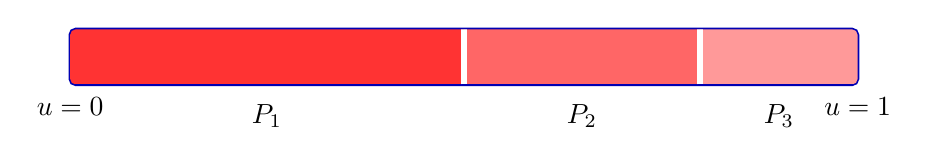
\begin{tikzpicture}[x=10cm,y=1cm]
      %=== parameters ===
      \def\h{0.35}          % half-height of the bar
      \def\r{2pt}           % corner radius for the outline/clip
      \def\pOne{0.50}       % P1 length in [0,1]
      \def\pTwo{0.30}       % P2 length in [0,1]
      \def\pThree{0.20}     % P3 length in [0,1] (should make p1+p2+p3=1)
    
      %=== background outline ===
      \draw[very thick, rounded corners=\r, blue!70!black]
        (0,-\h) rectangle (1,\h);
    
      %=== fill the three segments (clipped to rounded rectangle) ===
      \begin{scope}
        \clip[rounded corners=\r] (0,-\h) rectangle (1,\h);
        \fill[red!80!white]   (0,-\h)              rectangle (\pOne,\h);
        \fill[red!60!white]    (\pOne,-\h)          rectangle (\pOne+\pTwo,\h);
        \fill[red!40!white]   (\pOne+\pTwo,-\h)    rectangle (1,\h);
        % thin separators between segments
        \draw[line width=2pt,white] (\pOne,-\h) -- (\pOne,\h);
        \draw[line width=2pt,white] (\pOne+\pTwo,-\h) -- (\pOne+\pTwo,\h);
      \end{scope}
    
      %=== labels ===
      \node[anchor=north] at (0,-.4) {$u=0$};
      \node[anchor=north] at (1,-.4) {$u=1$};
    
      \node at (0.5*\pOne, -0.75) {$P_1$};
      \node at (\pOne+0.5*\pTwo, -0.75) {$P_2$};
      \node at (\pOne+\pTwo+0.5*\pThree, -0.75) {$P_3$};
    \end{tikzpicture}
    \caption{Sampling from a discrete distribution using a uniform random number. The interval $[0,1]$ is split into segments of lengths $P_i$; the outcome is determined by where $u\sim\mathcal U(0,1)$ lands.}
    \label{fig:discrete-sampling}
\end{figure}

\subsection{\texorpdfstring{Distances Between Distributions\textsuperscript{*}}{Distances Between Distributions}}
In many applications, especially in statistics and machine learning\footnote{For example, generative modeling objectives (MLE, VAEs, GANs, WGANs, diffusion) are built around specific divergences/distances (KL, JS, Wasserstein, Fisher).}, we need to quantify how different two probability distributions, $p_{\mathsf{x}}(x)$ and $q_{\mathsf{x}}(x)$, are. This turns a modeling question into a geometric one: how far is our model's predictive law $q_{\mathsf{x}}$ from the data-generating law $p_{\mathsf{x}}$? A first note is that some notions are true metrics\footnote{We mean this in a formal mathematical sense (see \href{https://en.wikipedia.org/wiki/Metric_(mathematics)}{Wikipedia} if this term is new to you and you're curious).} (non-negative, symmetric, and obeying the triangle inequality) while others are asymmetric divergences that act more like directional penalties. Choosing between them induces different learning behaviors and different numerical estimators.

\paragraph*{\texorpdfstring{Kullback-Leibler Divergence\textsuperscript{*}}{Kullback-Leibler Divergence}} The Kullback-Leibler divergence is the canonical asymmetric example. In the continuous case, it is defined as
\begin{equation}
    D_{\mathrm{KL}}(p_{\mathsf{x}}\Vert q_{\mathsf{x}})=\int p_{\mathsf{x}}(x)\log\!\left(\frac{p_{\mathsf{x}}(x)}{q_{\mathsf{x}}(x)}\right)\,dx
\end{equation}
it measures the expected extra log-loss incurred when coding samples from $p_{\mathsf{x}}$ with a code optimized for $q_{\mathsf{x}}$. Because the expectation is taken under $p_{\mathsf{x}}$, regions where $p_{\mathsf{x}}$ assigns mass but $q_{\mathsf{x}}$ is small are penalized heavily; if $q_{\mathsf{x}}(x)=0$ on a set where $p_{\mathsf{x}}(x)>0$, the divergence is infinite. The reverse divergence, $D_{\mathrm{KL}}(q_{\mathsf{x}}\Vert p_{\mathsf{x}})$, flips this emphasis and tends to be “mode-seeking,” preferring to place $q_{\mathsf{x}}$'s mass on a subset of $p_{\mathsf{x}}$'s high-density regions rather than cover all of $p_{\mathsf{x}}$.


\begin{exampleBox}
    \textbf{Example: Bernoulli and Gaussian KL Divergence}
    
    \emph{Bernoulli case:} For Bernoulli distributions with success probabilities $\theta_p$ and $\theta_q$,
    \begin{equation}
        D_{\mathrm{KL}}(\mathrm{Bernoulli}(\theta_p)\Vert \mathrm{Bernoulli}(\theta_q))
        =\theta_p\log\!\left(\frac{\theta_p}{\theta_q}\right)+(1-\theta_p)\log\!\left(\frac{1-\theta_p}{1-\theta_q}\right)
    \end{equation}
    Note that swapping $p_{\mathsf{x}}$ and $q_{\mathsf{x}}$ gives a generally different number like we expect since KL divergence is asymmetric. 

    \begin{figure}[H]
        \centering
        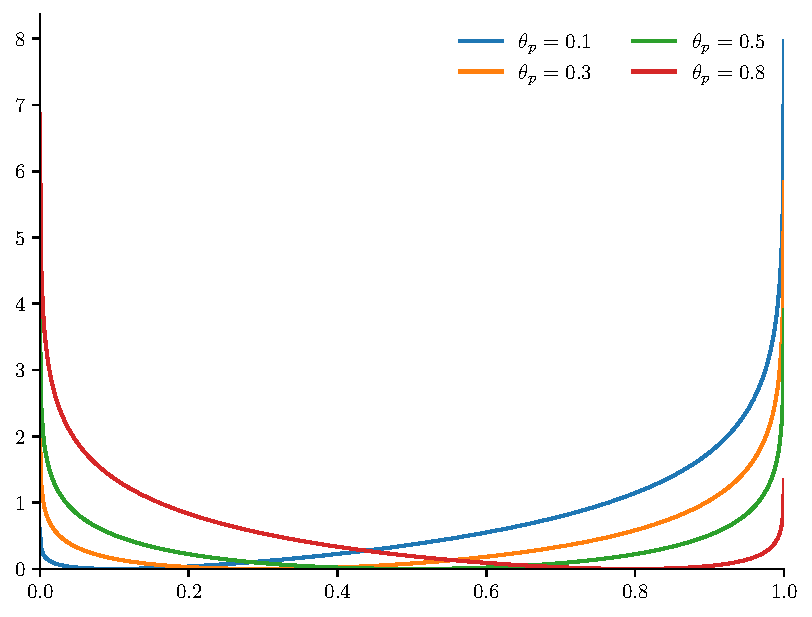
\includegraphics[width=0.4\textwidth]{figs/probability/bernoulli_kl_theta.pdf}
        \caption{For several fixed $\theta_p$, the curve shows $D_{\mathrm{KL}}(\mathrm{Bernoulli}(\theta_p)\Vert \mathrm{Bernoulli}(\theta_q))$ as $\theta_q$ varies. The divergence is minimized at $\theta_q=\theta_p$ and rises sharply as $\theta_q\to 0$ (if $\theta_p\neq 0$) or $\theta_q\to 1$ (if $\theta_p \neq 1$) since there is an enormous penalty for assigning near-zero probability to outcomes that $p$ deems likely. Different $\theta_p$ produce different profiles since KL is directional and depends on which distribution is treated as $p$.}
        \label{fig:bernoulli-kl-theta}
    \end{figure}

    \emph{Gaussian case:} In Gaussian families, we also have a closed form for the KL divergence. If $p_{\mathsf{x}}=\mathcal{N}(\mu_p,\sigma_p^2)$ and $q_{\mathsf{x}}=\mathcal{N}(\mu_q,\sigma_q^2)$,
    \begin{equation}
        D_{\mathrm{KL}}(p_{\mathsf{x}}\Vert q_{\mathsf{x}})=\frac{1}{2}\!\left(\frac{\sigma_p^2}{\sigma_q^2}+\frac{(\mu_q-\mu_p)^2}{\sigma_q^2}-1+\log\!\left(\frac{\sigma_q^2}{\sigma_p^2}\right)\right)
    \end{equation}

    \begin{figure}[H]
        \centering
        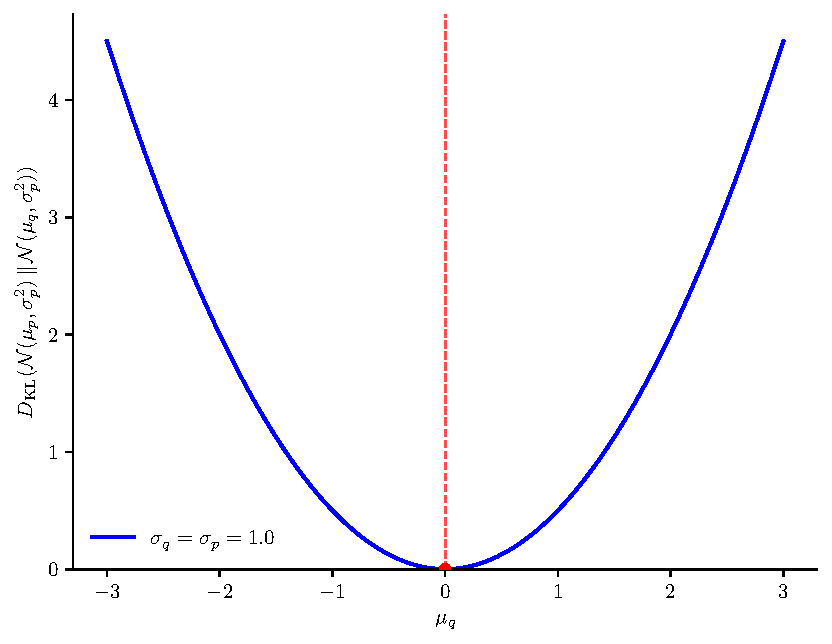
\includegraphics[width=0.4\textwidth]{figs/probability/gaussian_kl_mu.pdf}
        \caption{With equal variances $\sigma_p^2=\sigma_q^2 = \sigma^2$, the KL reduces to $\tfrac{1}{2}(\mu_q-\mu_p)^2/\sigma^2$. The plot is a convex parabola in $\mu_q$ with a unique minimum of $0$ at $\mu_q=\mu_p$; the cost grows quadratically with mean error and is inversely scaled by the variance.}
        \label{fig:gaussian-kl-mu-sigma}
    \end{figure}
\end{exampleBox}
    
\paragraph*{\texorpdfstring{Jensen-Shannon Divergence\textsuperscript{*}}{Jensen-Shannon Divergence}} For a symmetric, bounded alternative closely related to KL, we can use the Jensen-Shannon divergence:
\begin{equation}
    \mathrm{JSD}(p_{\mathsf{x}},q_{\mathsf{x}})=\frac12 D_{\mathrm{KL}}(p_{\mathsf{x}}\Vert m_{\mathsf{x}})+\frac12 D_{\mathrm{KL}}(q_{\mathsf{x}}\Vert m_{\mathsf{x}}), \quad m_{\mathsf{x}}=\frac12(p_{\mathsf{x}}+q_{\mathsf{x}})
\end{equation}
It behaves like a metric (its square root is a true metric) and remains finite even when supports do not. This is used in text, image, and generative-model comparisons.

\paragraph*{\texorpdfstring{Wasserstein Distance\textsuperscript{*}}{Wasserstein Distance}} Optimal-transport distances, or Wasserstein metrics, take a geometric view of discrepancy: they measure the minimal work needed to move one distribution into another by transporting probability mass through space. Concretely, if moving unit mass from $x$ to $y$ costs $c(x,y)=|x-y|^p$, the $p$-Wasserstein distance is
\begin{equation}
    W_p(p_{\mathsf{x}},q_{\mathsf{x}})=\left(\inf_{\gamma\in\Gamma(p_{\mathsf{x}},q_{\mathsf{x}})}\int |x-y|^p\,d\gamma(x,y)\right)^{1/p}
\end{equation}
where $\Gamma(p_{\mathsf{x}},q_{\mathsf{x}})$ is the set of couplings with marginals $p_{\mathsf{x}}$ and $q_{\mathsf{x}}$. In one dimension, this becomes especially tangible because the 1-Wasserstein distance equals the $L^1$ distance between the cumulative distribution functions:
\begin{equation}
    W_1(p_{\mathsf{x}},q_{\mathsf{x}})=\int_{-\infty}^{\infty}|F_p(t)-F_q(t)|\,dt
\end{equation}
(Very importantly, this allows for a simple sample estimator by sorting observations and comparing empirical quantiles.) For Gaussian laws, there are also closed forms for the squared 2-Wasserstein distance:
\begin{equation}
    W_2^2\big(\mathcal{N}(\mu_p,\sigma_p^2),\mathcal{N}(\mu_q,\sigma_q^2)\big)=(\mu_p-\mu_q)^2+(\sigma_p-\sigma_q)^2
\end{equation}
In higher dimensions, the formula involves matrix square roots:
\begin{equation}
    W_2^2\big(\mathcal{N}(\boldsymbol{\mu}_1,\boldsymbol{\Sigma}_1),\mathcal{N}(\boldsymbol{\mu}_2,\boldsymbol{\Sigma}_2)\big)=\|\boldsymbol{\mu}_1-\boldsymbol{\mu}_2\|^2+\mathrm{Tr}\!\left(\boldsymbol{\Sigma}_1+\boldsymbol{\Sigma}_2-2\!\left(\boldsymbol{\Sigma}_2^{1/2}\boldsymbol{\Sigma}_1\boldsymbol{\Sigma}_2^{1/2}\right)^{1/2}\right)
\end{equation}
This version has become a staple in comparing embeddings and generative models. Indeed, its optimal-transport foundation makes it especially useful in normalizing flows and diffusion models, where it gives robust, physically interpretable discrepancies between distributions (even with support mismatch!) and connects learning to Fokker-Planck/Schr\"odinger bridge dynamics. These types of models are extremely popular in current research (image/video/audio/small molecule generation, etc.).

\paragraph*{\texorpdfstring{Kolmogorov-Smirnov Statistic\textsuperscript{*}}{Kolmogorov-Smirnov Statistic}} When the goal is hypothesis testing rather than a continuous measure of discrepancy, we can use the Kolmogorov-Smirnov statistic to compare cumulative distribution functions. Given a sample $\mathsf{x}_{1:n}$ from $p_{\mathsf{x}}$, with empirical CDF $F_n$, and a fully specified theoretical CDF $F_0$ for $q_{\mathsf{x}}$, the one-sample statistic is 
\begin{equation}
    D_n=\sup_x |F_n(x)-F_0(x)|
\end{equation}
That is, it's the maximum vertical gap between the empirical and theoretical CDFs. Large values indicate a poor fit. Because KS looks only at CDF gaps, it is most sensitive near the median and can miss tail differences. If tail sensitivity is important, one might instead consider something like the Cram\'er-von Mises or Anderson-Darling statistics, which reweight discrepancies, though these require more setup than KS's simple sup-norm.


%%% Local Variables:
%%% mode: LaTeX
%%% TeX-master: "../main"
%%% End: